\documentclass[zavrsni, numeric]{fer}
\usepackage{booktabs}
\usepackage[section]{placeins}
\usepackage{float}


\begin{document}

\thesisnumber{5375}

\title{Programska podrška za svršenike}

\author{Tomislav Kravaršćan}

\maketitle
 
\tableofcontents

\chapter{Uvod}
Svršenici (lat. \textit{alumni}) je popularan naziv za bivše pripadnike neke ustanove, najčešće sveučilišta. Alumni su uobičajena udruženja u svijetu pa u nekim sveučilištima imaju i stoljetnu tradiciju. Njihovo ponovno okupljanje i sudjelovanje u radu sveučilišta je vrlo bitno za održavanje priče o prošlosti, a i za planiranje budućnosti sveučilišta. No, kako studenti sveučilišta vrlo brzo nakon diplomiranja utonu u nove životne prilike kao što su posao i obitelj, fakultetima je vrlo teško održavati vezu sa svojim bivšim studentima i ponovno ih okupljati. A i sami se svršenici teško održe na okupu. Za to je rješenje programska podrška u obliku informacijske web aplikacije, gdje će se moći organizirati događaji, sastanci i objavljivati razne objave vezane za svršenike.

\chapter{Analiza postojeće programske podrške}
Analizom postojeće programske potpore nastojimo bolje razumijeti problem koji rješavamo, njegovu domenu primjene i razrješiti moguće krive početne pretpostavke o programskoj podršci koju izrađujemo. Također, jasnije vidimo funkcionalnosti koje bi trebali implementirati i dobivamo ideje o nekim detaljima o kojima uopće nismo razmišljali. Osim toga, svrha analize je i otrkivanje mogućih nedostataka koje trpi posojeća programska podrška, te učenje na tuđim pogreškama. Moramo biti posebno svjesni kojim su resursima raspolagali razvojni inženjeri analiziranih rješenja kako bismo što ranije odredili doseg našeg rješenja sukladno našim resursima vremena i znanja.
U ovom konkretnom slučaju, analizirati ćemo programska rješenja za upravljanje svršenicima. Takvih rješenja ima neiscrpno puno pa ćemo navesti samo neka od njih. Gotovo sva postojeća rješenja nude neke osnovne funkcionalnosti kao što su organizacija i pregled događaja, pregled novosti, informacije o sustavu, ponuda poslova, stvaranje i upravljanje korisničkim računom.

\section{Graduway}
Graduway[1] je web platforma istoimene tvrtke koja za različite fakultete po narudžbi stvara aplikaciju prilagođenu određenoj ustanovi za koju se izrađuje. Uz gore navedene osnovne funkcionalnosti ovakvog i sličnih rješenja, Graduway ima još puno funkcionalnosti kao što su adminske stranice, pregled statistike korisnika i vizualizacija itd. Dostupna je za isporuku na iOS, Android ili kao web- aplikacija.

Neki od njihovih klijenata za rješenje upravljanja svršenicima su Longwood University, University of Dundee, Brunel University, UCLA i mnogi drugi.

Svako rješenje je napravljeno za preko tisuću korisnika, početna cijena je pet tisuća dolara godišnje, te je ponuđen besplatni probni period.

\begin{figure}[H]
	\centering
	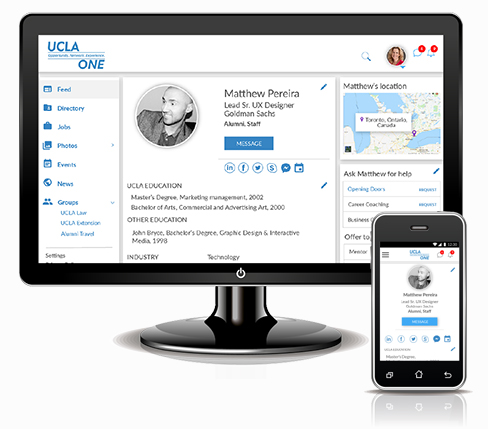
\includegraphics[width=13cm]{slike/izgledUCLAgraduwayRjesenja.png}
	\caption{Izgled UCLA Graduway rješenja}
	\label{fig:ucla-graduway}
\end{figure}

\section{VeryConnect}
VeryConnect je nešto manje popularna platforma za upravljanje svršenicima, ali sa jednako opširnim funkcionalnostima. Ima znatno manji broj klijenata od kojih je samo jedno sveučilište, University of Glasgow. Također ima neku početnu cijenu koja za razliku od Graduway-a nije javno vidljiva, a dodatne funkcionalnosti se naplaćuju zasebno.

\begin{figure}[H]
	\centering
	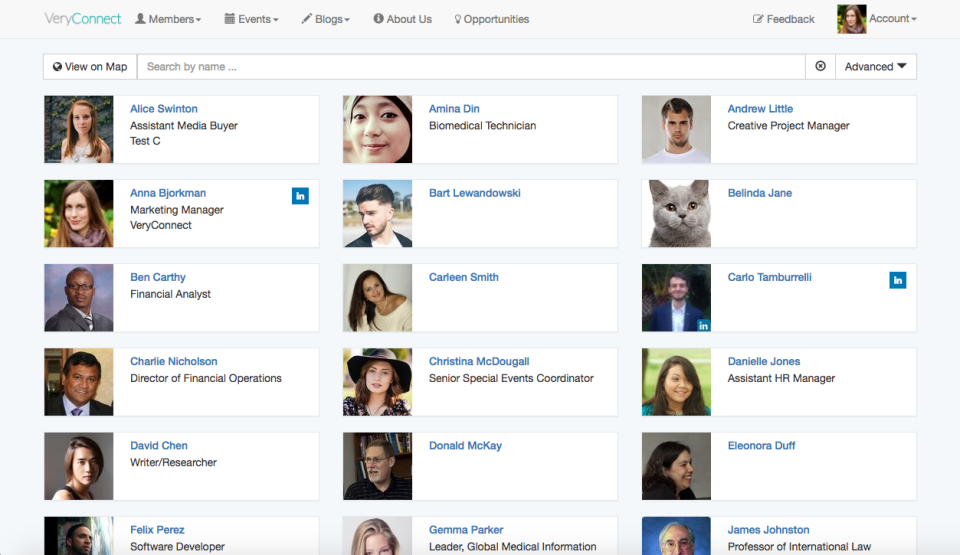
\includegraphics[width=13cm]{slike/very-connect-korisnici.png}
	\caption{VeryConnect - pregled korisnika}
	\label{fig:veryconn-users}
\end{figure}

\begin{figure}[H]
	\centering
	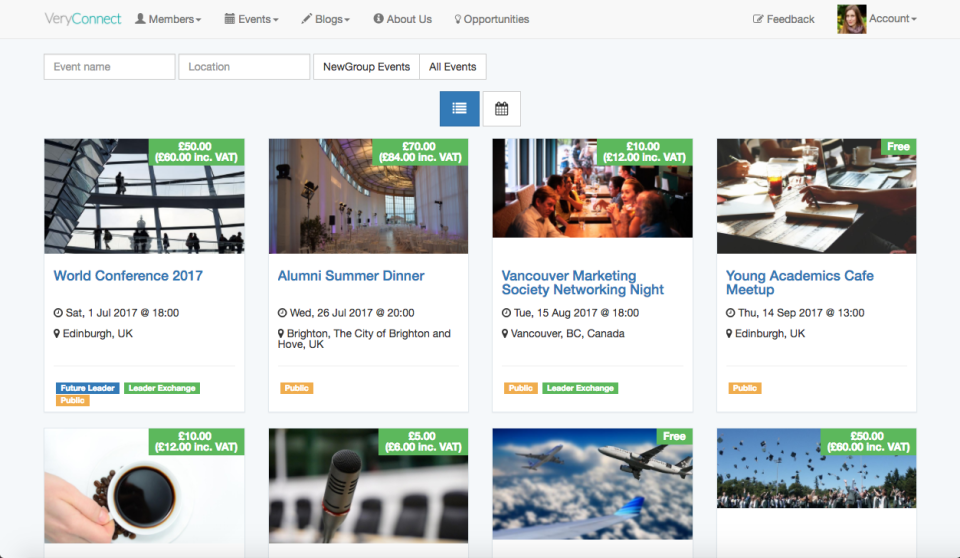
\includegraphics[width=13cm]{slike/very-connect-dogadaji.png}
	\caption{VeryConnect - pregled događaja}
	\label{fig:veryconn-events}
\end{figure}

\section{Hiverbrite}
Hiverbrite je također platforma sa vrlo opširnim funkcionalnostima.

\begin{figure}[H]
	\centering
	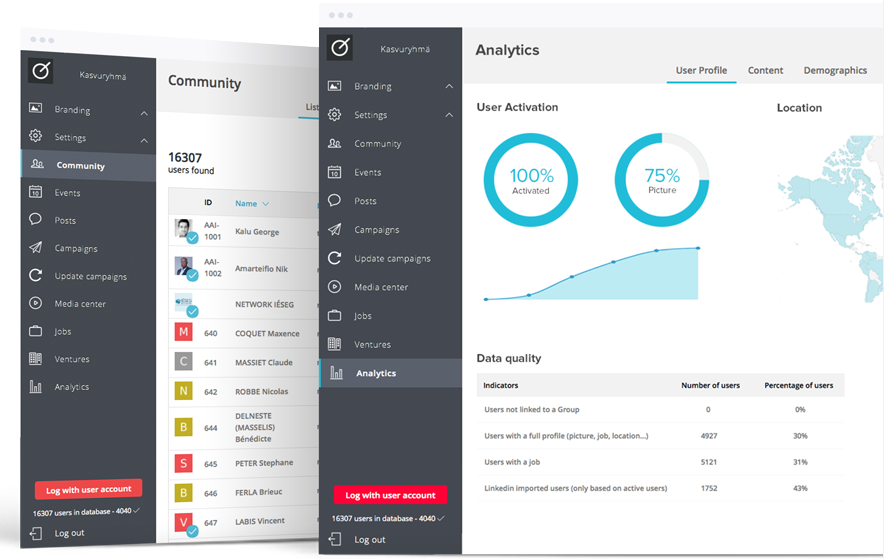
\includegraphics[width=13cm]{slike/hiverbrite-upravljanje.png}
	\caption{Izgled Hiverbrite stranice za upravljanje zajednicom}
	\label{fig:hiverbrite-menagements}
\end{figure}

\chapter{Zahtjevi nad programskom potporom}
Zahtjevi nad programskom potporom dijele se na funkcionalne zahtjeve – ono što korisnik očekuje od sustava i osnovne potrebe zbog kojih korisnik želi programsku potporu, te nefunkcionalne zahtjeve – ograničenja sustava i način na koji sustav treba biti izveden.

\section{Funkcionalni zahtjevi}
Funkcionalni zahtjevi su izjavljeni u prirodnom jeziku u obliku slučajeva korištenja, forma svakog slučaja korištenja: naziv slučaja korištenja – glavni sudionik.

 
\begin{itemize}
	\item Pregled postova - korisnik
	\item Pregled arhive postova - korisnik
	\item Filtriranje postova po kategoriji - korisnik
	\item Dodavanje posta - administrator
	\item Brisanje posta - administrator
	\item Uređivanje posta - administrator
	\item Pregled korisničkog računa - korisnik
	\item Dodavanje korisničkog računa (registracija) - anonimni korisnik
	\item Brisanje korisničkog računa - korisnik 
	\item Uređivanje korisničkog računa - korisnik
	\item Pregled svih korisnika - administrator
	\item Prijava na sustav - korisnik 
	\item Odjava sa sustava - korisnik
	\item Preplata na kategoriju - korisnik
	\item Otkazivanje pretplate na kategoriju - korisnik
	\item Slanje pošte obavijesti prilikom objave novog posta - aplikacija
\end{itemize}

\section{Nefunkcionalni zahtjevi}
Nefunkcionalni zahtjevi su sljedeći:

\begin{itemize}
	\item Sustav mora podržavati istodobni rad više korisnika
	\item Sustav mora biti otporan na kritične pogreške
	\item Sustav mora biti otporan na \textit{Cross site scripting - XSS}\citep{xss} ranjivosti
	\item Sustav mora biti ostvaren model-pogled-upravljač (eng. \textit{Model-View-Controller - MVC}) arhitekturom kao web aplikacija
	\item Sustav mora biti u mogućnosti spremati podatke u bazu podataka
\end{itemize}

\chapter{Arhitektura sustava}
\section{Baza podataka}
\subsection{Fizički model baze podataka}

\begin{figure}[H]
	\centering
	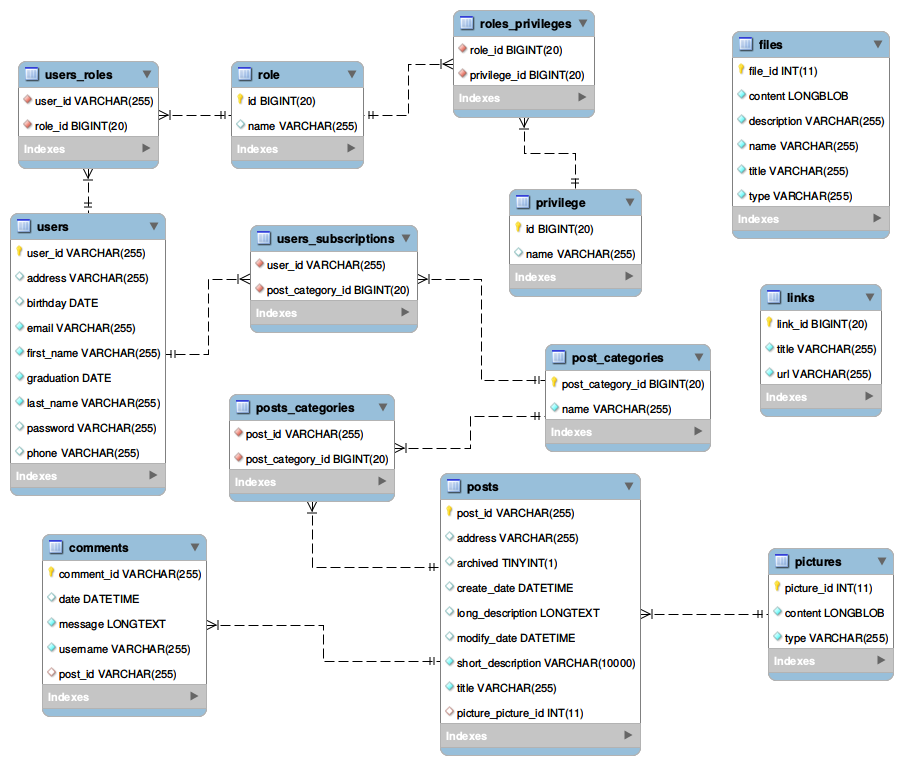
\includegraphics[width=13cm]{slike/fizicki-model.png}
	\caption{Fizički model baze podataka}
	\label{fig:fizicki-model}
\end{figure}

\subsection{Opis tablica}

\subsubsection{Users}

\begin{figure}[H]
	\centering
	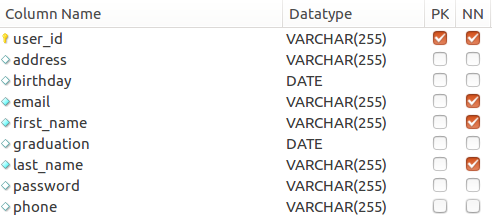
\includegraphics[width=7cm]{slike/t-users.png}
	\caption{Tablica Users}
	\label{fig:t-users}
\end{figure}

U tablici \textit{Users} su podaci o korisnicima aplikacije. Polja email, ime, prezime i lozinka su nužna za rad aplikacije, pa imaju "NN", odnosno \textit{Not Null} oznaku.

\subsubsection{Roles}

\begin{figure}[H]
	\centering
	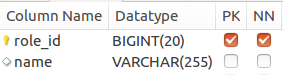
\includegraphics[width=7cm]{slike/t-roles.png}
	\caption{Tablica Roles}
	\label{fig:t-roles}
\end{figure}

Tablica \textit{Roles} nam služi za spremanje uloga korisnika u bazu. Pomoću tih uloga aplikacija određuje dozvole nad određenim akcijama.

\subsubsection{Privileges}

\begin{figure}[H]
	\centering
	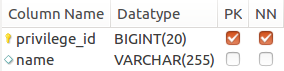
\includegraphics[width=7cm]{slike/t-privileges.png}
	\caption{Tablica Privileges}
	\label{fig:t-privileges}
\end{figure}

Tablica \textit{Privileges} služi istoj svrsi kao i tablica \textit{Roles}, samo što ova tablica pospješuje bolju granulaciju dozvola nad akcijama koje korisnik može obaviti u aplikaciji.

\subsubsection{Users roles}

\begin{figure}[H]
	\centering
	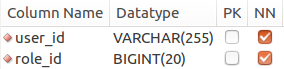
\includegraphics[width=7cm]{slike/t-users_roles.png}
	\caption{Tablica Users roles}
	\label{fig:t-users_roles}
\end{figure}

Svaki korisnik može imati više uloga, a svaka uloga može biti zastupljena kod više korisnika. Ova tablica spaja ta dva entiteta.

\subsubsection{Roles privileges}

\begin{figure}[H]
	\centering
	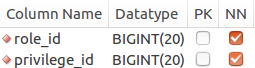
\includegraphics[width=7cm]{slike/t-roles_privileges.png}
	\caption{Tablica Roles privileges}
	\label{fig:t-roles_privileges}
\end{figure}

Svaka uloga može imati više privilegija, te svaka privilegija može biti prisutna u više uloga. Zbog toga postoji ova tablica koja spaja uloge sa privilegijama.

\subsubsection{Posts}

\begin{figure}[H]
	\centering
	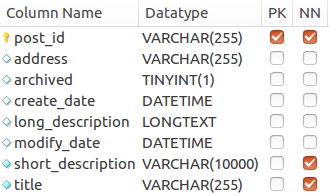
\includegraphics[width=7cm]{slike/t-posts.png}
	\caption{Tablica Posts}
	\label{fig:t-posts}
\end{figure}

Tablica \textit{Posts} sprema podatke o postovima. Podaci koji su nužni su naslov i kratki opis. Datum izrade posta se automatski sprema u bazu prilikom \textit{Insert} akcije, dok se datum izmjene automatski ažurira prilikom \textit{Update} akcije.

\subsubsection{Post categories}

\begin{figure}[H]
	\centering
	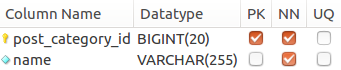
\includegraphics[width=7cm]{slike/t-post_categories.png}
	\caption{Tablica Post categories}
	\label{fig:t-post_categories}
\end{figure}

Svaki post može imati više kategorija. Tablica \textit{Post categories} sprema te vrste kategorija. Ime kategorije je obavezno pa je označeno \textit{Not Null} oznakom.

\subsubsection{Posts categories}

\begin{figure}[H]
	\centering
	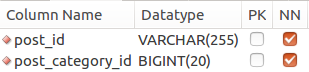
\includegraphics[width=7cm]{slike/t-posts_categories.png}
	\caption{Tablica Posts categories}
	\label{fig:t-posts_categories}
\end{figure}

Pošto svaki post može imati više kategorija, a svaka kategorija može biti prisutna u više postova, postoji tablica \textit{Posts categories} koja spaja ta dva entiteta.

\subsubsection{Users subscriptions}

\begin{figure}[H]
	\centering
	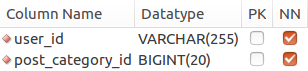
\includegraphics[width=7cm]{slike/t-users_subscriptions.png}
	\caption{Tablica Users subscriptions}
	\label{fig:t-users_subscriptions}
\end{figure}

Korisnik može biti pretplaćen na više kategorija, a više kategorija može biti u listi pretplata različitih korisnika. Zato tablica \textit{Users subscriptions} čuva informaciju o tome koji je korisnik pretplaćen na koje kategorije.

\subsubsection{Comments}

\begin{figure}[H]
	\centering
	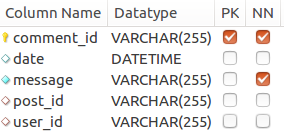
\includegraphics[width=7cm]{slike/t-comments.png}
	\caption{Tablica Comments}
	\label{fig:t-comments}
\end{figure}

Tablica \textit{Comments} sadrži podatke o komentarima na razne postove. Za komentar je bitno da u bazi bude prisutno ime autora komentara, te poruka koju komentar sadrži. Datum komentara se automatski upisuje prilikom \textit{Insert} akcije.

\subsubsection{Posts comments}

\begin{figure}[H]
	\centering
	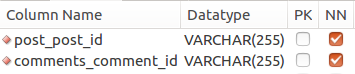
\includegraphics[width=7cm]{slike/t-posts_comments.png}
	\caption{Tablica Posts comments}
	\label{fig:t-posts_comments}
\end{figure}

Svaki post može imati više komentara, tablica \textit{Posts comments} sadrži podatke o tome koji post ima koje komentare.

\subsubsection{Links}

\begin{figure}[H]
	\centering
	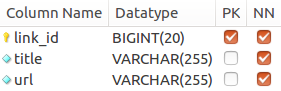
\includegraphics[width=7cm]{slike/t-links.png}
	\caption{Tablica Links}
	\label{fig:t-links}
\end{figure}

Tablica \textit{Links} sadrži ime i "URL" poveznica.

\section{Obrazac model-pogled-upravljač}
Obrazac jedan je od najčešće upotrebljavanih arhitekturnih obrazaca prilikom izrade web aplikacija. Glavna ideja obrasca je logičko i fizičko odvajanje poslovnih procesa, odnosno dobavljanja podataka i operacija nad njima, od prikaza tih podataka na klijentskoj strani aplikacije.  

U MVC obrascu, model predstavlja svojevrsno spremište podataka kojem mogu pristupiti ostala dva sudionika, upravljač i pogled. 

Upravljač je zadužen za obavljanje neke operacije. Svakom je upravljaču pridružen jedinstveni \textit{URL (Uniform Resource Locator)}. Najčešće pomoću repozitorija dohvaća podatke iz baze, odradi neku akciju nad njima i ubacuje ih u model. Nakon toga klijentu šalje neku vrstu odgovora, a taj odgovor je većinom stranica sa \textit{Hyper Text Markup Language - html} oznakama, odnosno pogled.

Pogled je \textit{html} datoteka koja prikazuje podatke na klijentskoj strani aplikacije. Izveden je tako da koristi neku tehnologiju kojom je moguće obavljati operacije nad podacima koji se nalaze u modelu. Takva tehnologija je programski jezik koji, kao i svaki drugi treba biti preveden prije slanja stranice klijentu. 

\subsection{Modeli podataka}
U ovoj aplikaciji su modeli podataka \textit{Java} razredi sa posebnim oznakama koje se mogu staviti iznad naziva polja lokalnih podataka, metoda za dobavljanje lokalnih podataka ili konstruktora. Te se oznake prilikom prevođenja koriste za stvaranje fizičkog modela baze podataka. Pomoću tih oznaka također je moguće vrlo detaljno opisati karakteristike podataka koji će fizički biti spremljeni. 

\subsection{Pogledi}
Pogledi i logika prikaza podataka je implementirana pomoću \textit{JSP(Java Server Pages)} tehnologije.

\subsection{Upravljači}
Upravljači su u ovoj aplikaciji implementirani pomoću \textit{Spring Boot} tehnologije. Pomoću te tehnologije je, slično kao i za model podataka, moguće definirati oznake kojima se prilikom prevođenja razredi i metode u aplikaciji povezuju s različitim URL-ovima.

\chapter{Implementirane funkcionalnosti}
Pregled funkcionalnosti koje posjeduje programska potpora. Svaka funkcionalnost je popraćena opisom i slikom koja pokazuje njenu implementaciju.

\section{Navigacijska traka}

\begin{figure}[H]
	\centering
	
\includegraphics[width=13cm]{slike/nav-admin.png}
	\caption{Navigacijska traka admistratora}
	\label{fig:nav-admin}
\end{figure}

Navigacijska traka je \textit{html} element koji se pojavljuje u svim \textit{html} stranicama aplikacije i svrha joj je omogućavanje dolaska do svih stranica aplikacije. Svaki korisnik putem navigacijske trake u svakom trenutku može doći do početne stranice, gdje je popis svih postova, odabirom "Alumni" natpisa u lijevom dijelu trake. 

\subsection{Navigacijska traka za anonimnog(ne prijavljenog) korisnika}
Anonimni korisnik pomoću navigacijske trake može doći do stranice za registraciju, stranice za prijavu te ima pregled svih poveznica koje su u sustavu. 

\subsection{Navigacijska traka za prijavljenog korisnika}
Prijavljenom se korisniku više ne prikazuje mogućnost odabira prijave niti registracije, nego u desnom dijelu trake ima prikaz svoga imena kojeg može odabrati. Tim odabirom mu se prikazuje padajući izbornik koji prikazuje dvije dodatne opcije, prikaz vlastitog profila, te odjava sa sustava.

Navigacijska traka je posebno bitna i administratoru sustava, koji, ako je prijavljen, vidi dodatnu opciju odabira padajućeg izbornika "Admin", čijim odabirom se otvara padajući izbornik sa opcijama izrade novog posta, pregleda arhive postova, svih korisnika, kategorija te poveznica.

\subsection{Registracija na sustav}

\begin{figure}[H]
	\centering
	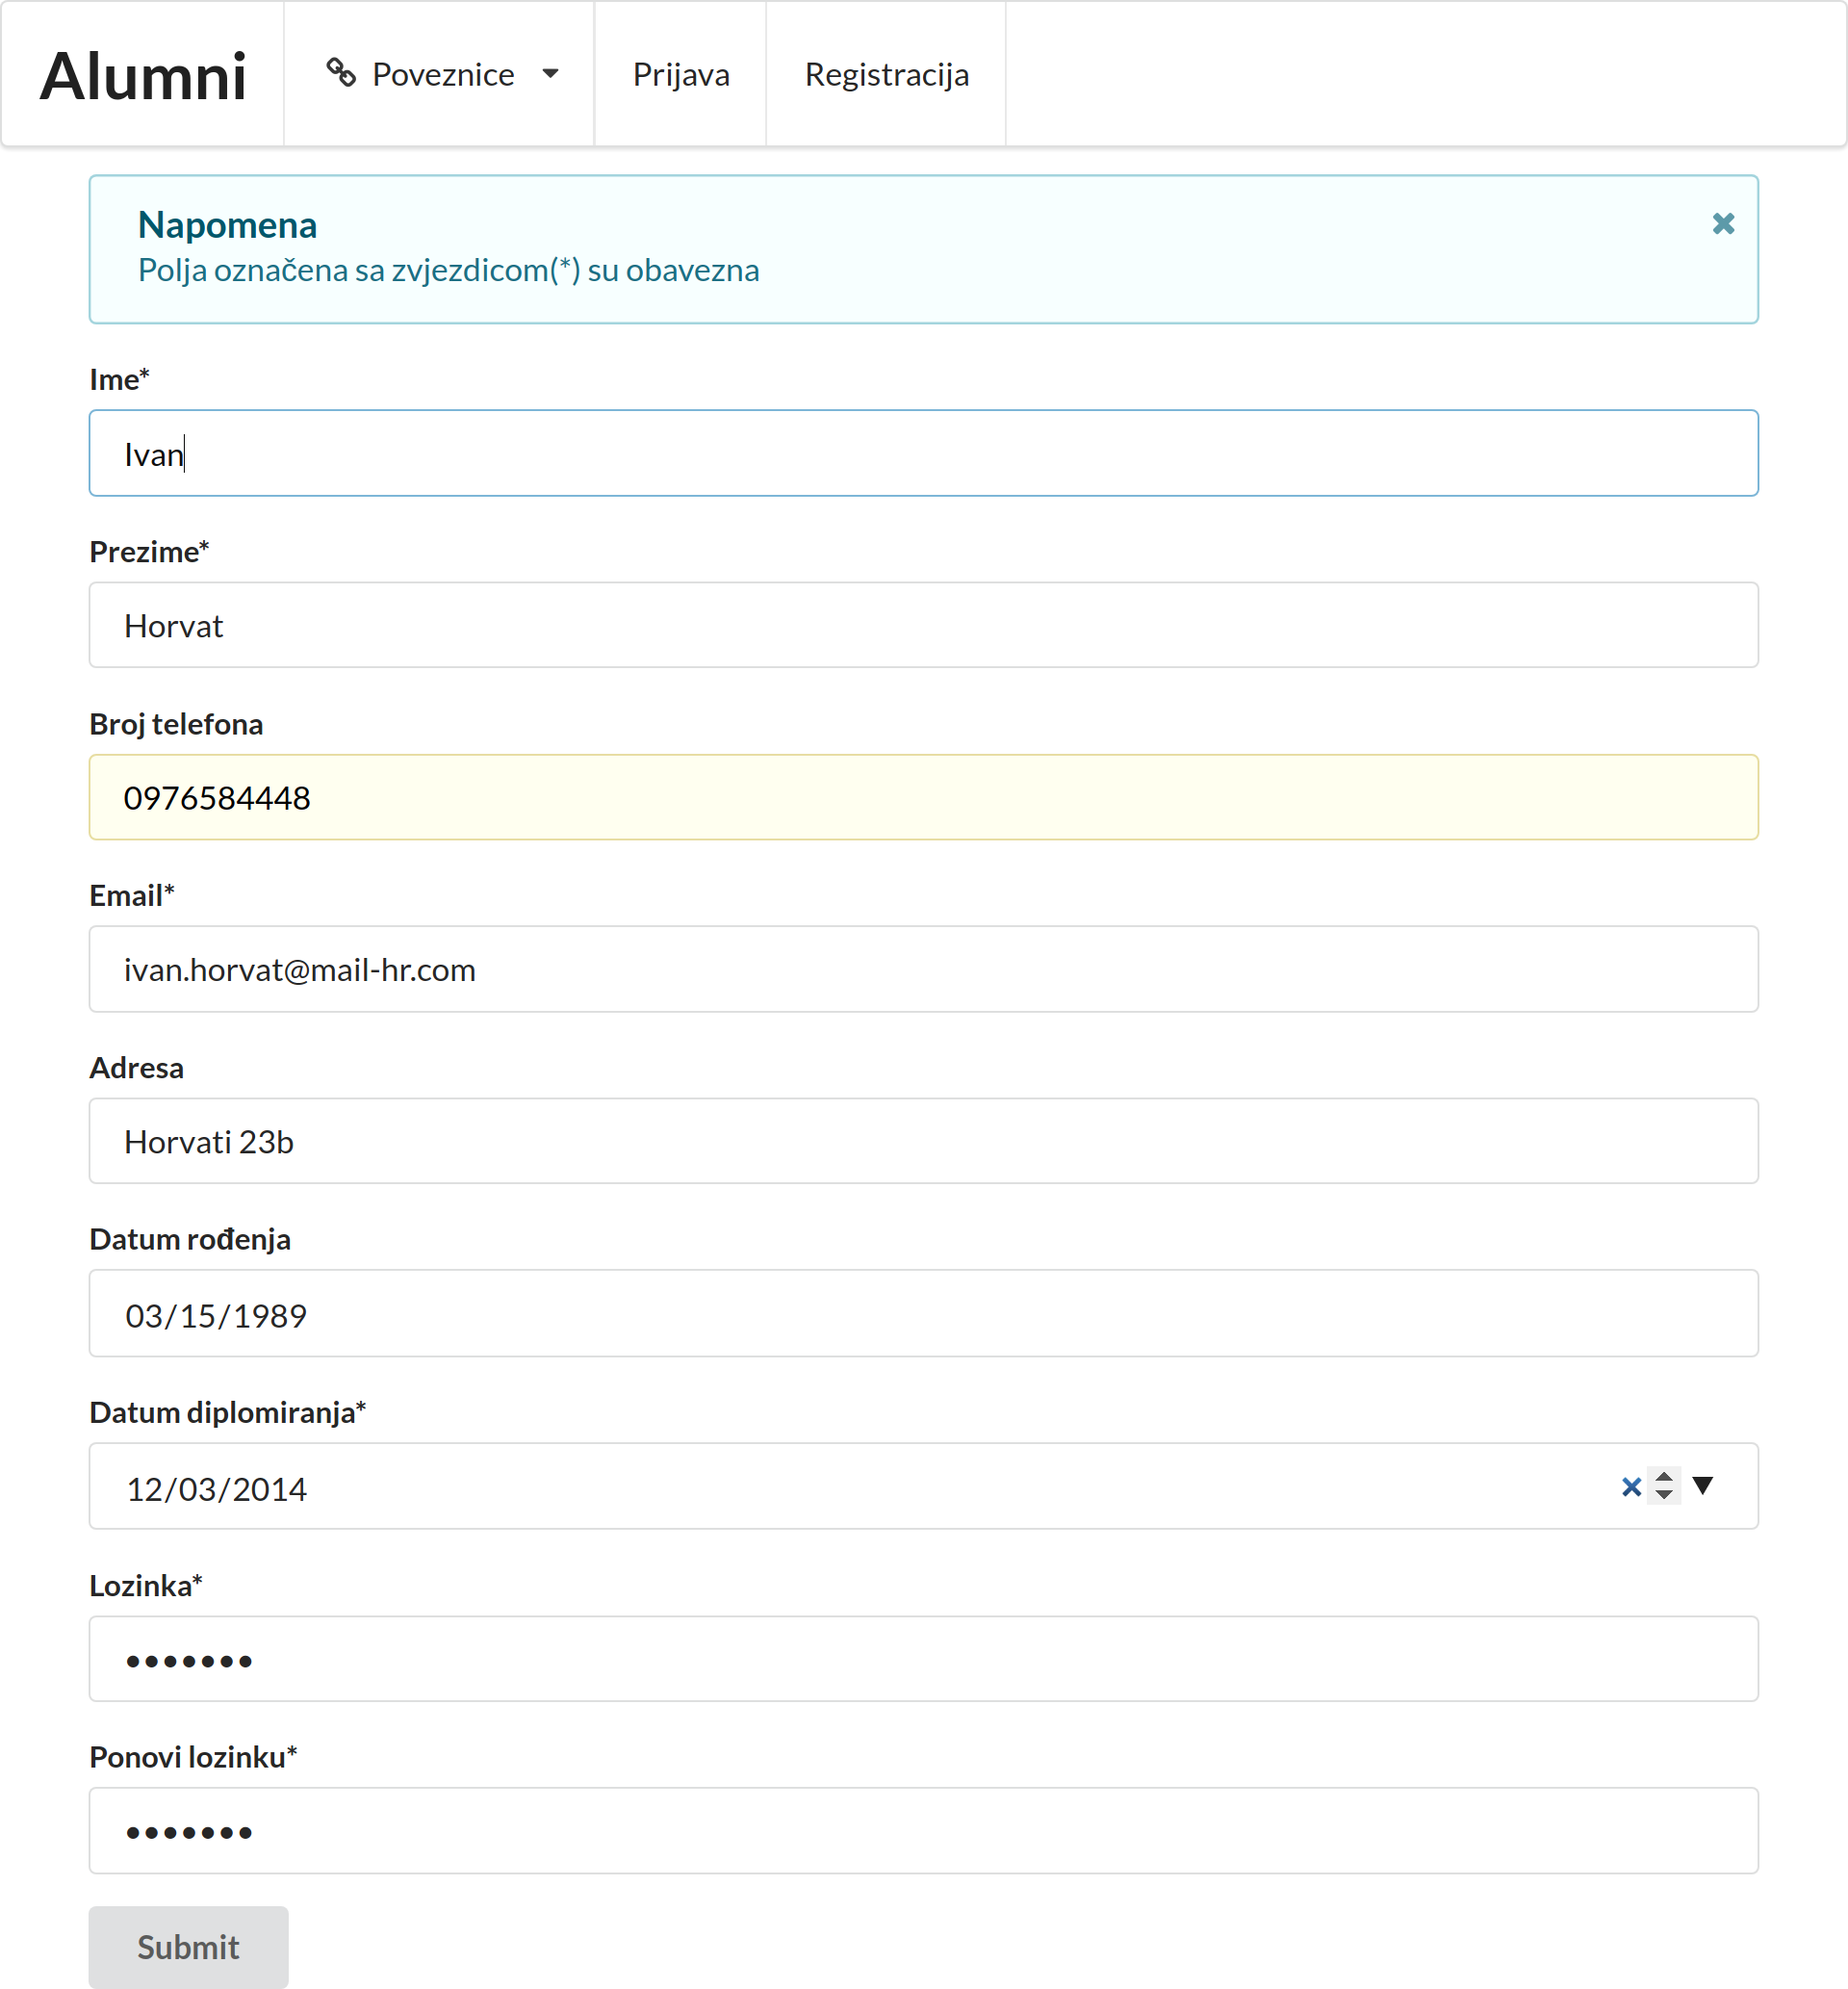
\includegraphics[width=13cm]{slike/registracija.png}
	\caption{Obrazac za registraciju}
	\label{fig:registracija}
\end{figure}

Prilikom odabira opcije "Registracija" u navigacijskoj traci, anonimnom se korisniku prikaže obrazac za registraciju na sustav. Kako bi se uspješno registrirao, korisnik mora upisati ime, prezime, email, datum diplomiranja te lozinku. Broj telefona, adresa i datum rođenja su neobavezna polja te se korisniku daje na izbor hoće li ih upisati ili ne. Za sve navedene obavezne stavke postoje provjere na klijentskoj te na poslužiteljskoj strani, te osim provjera za postojanost obaveznih stavki, postoje i provjere za ispravnost email-a, te provjere da li lozinka ima najmanje 6, a najviše 30 znakova.

\subsection{Prijava na sustav}

\begin{figure}[H]
	\centering
	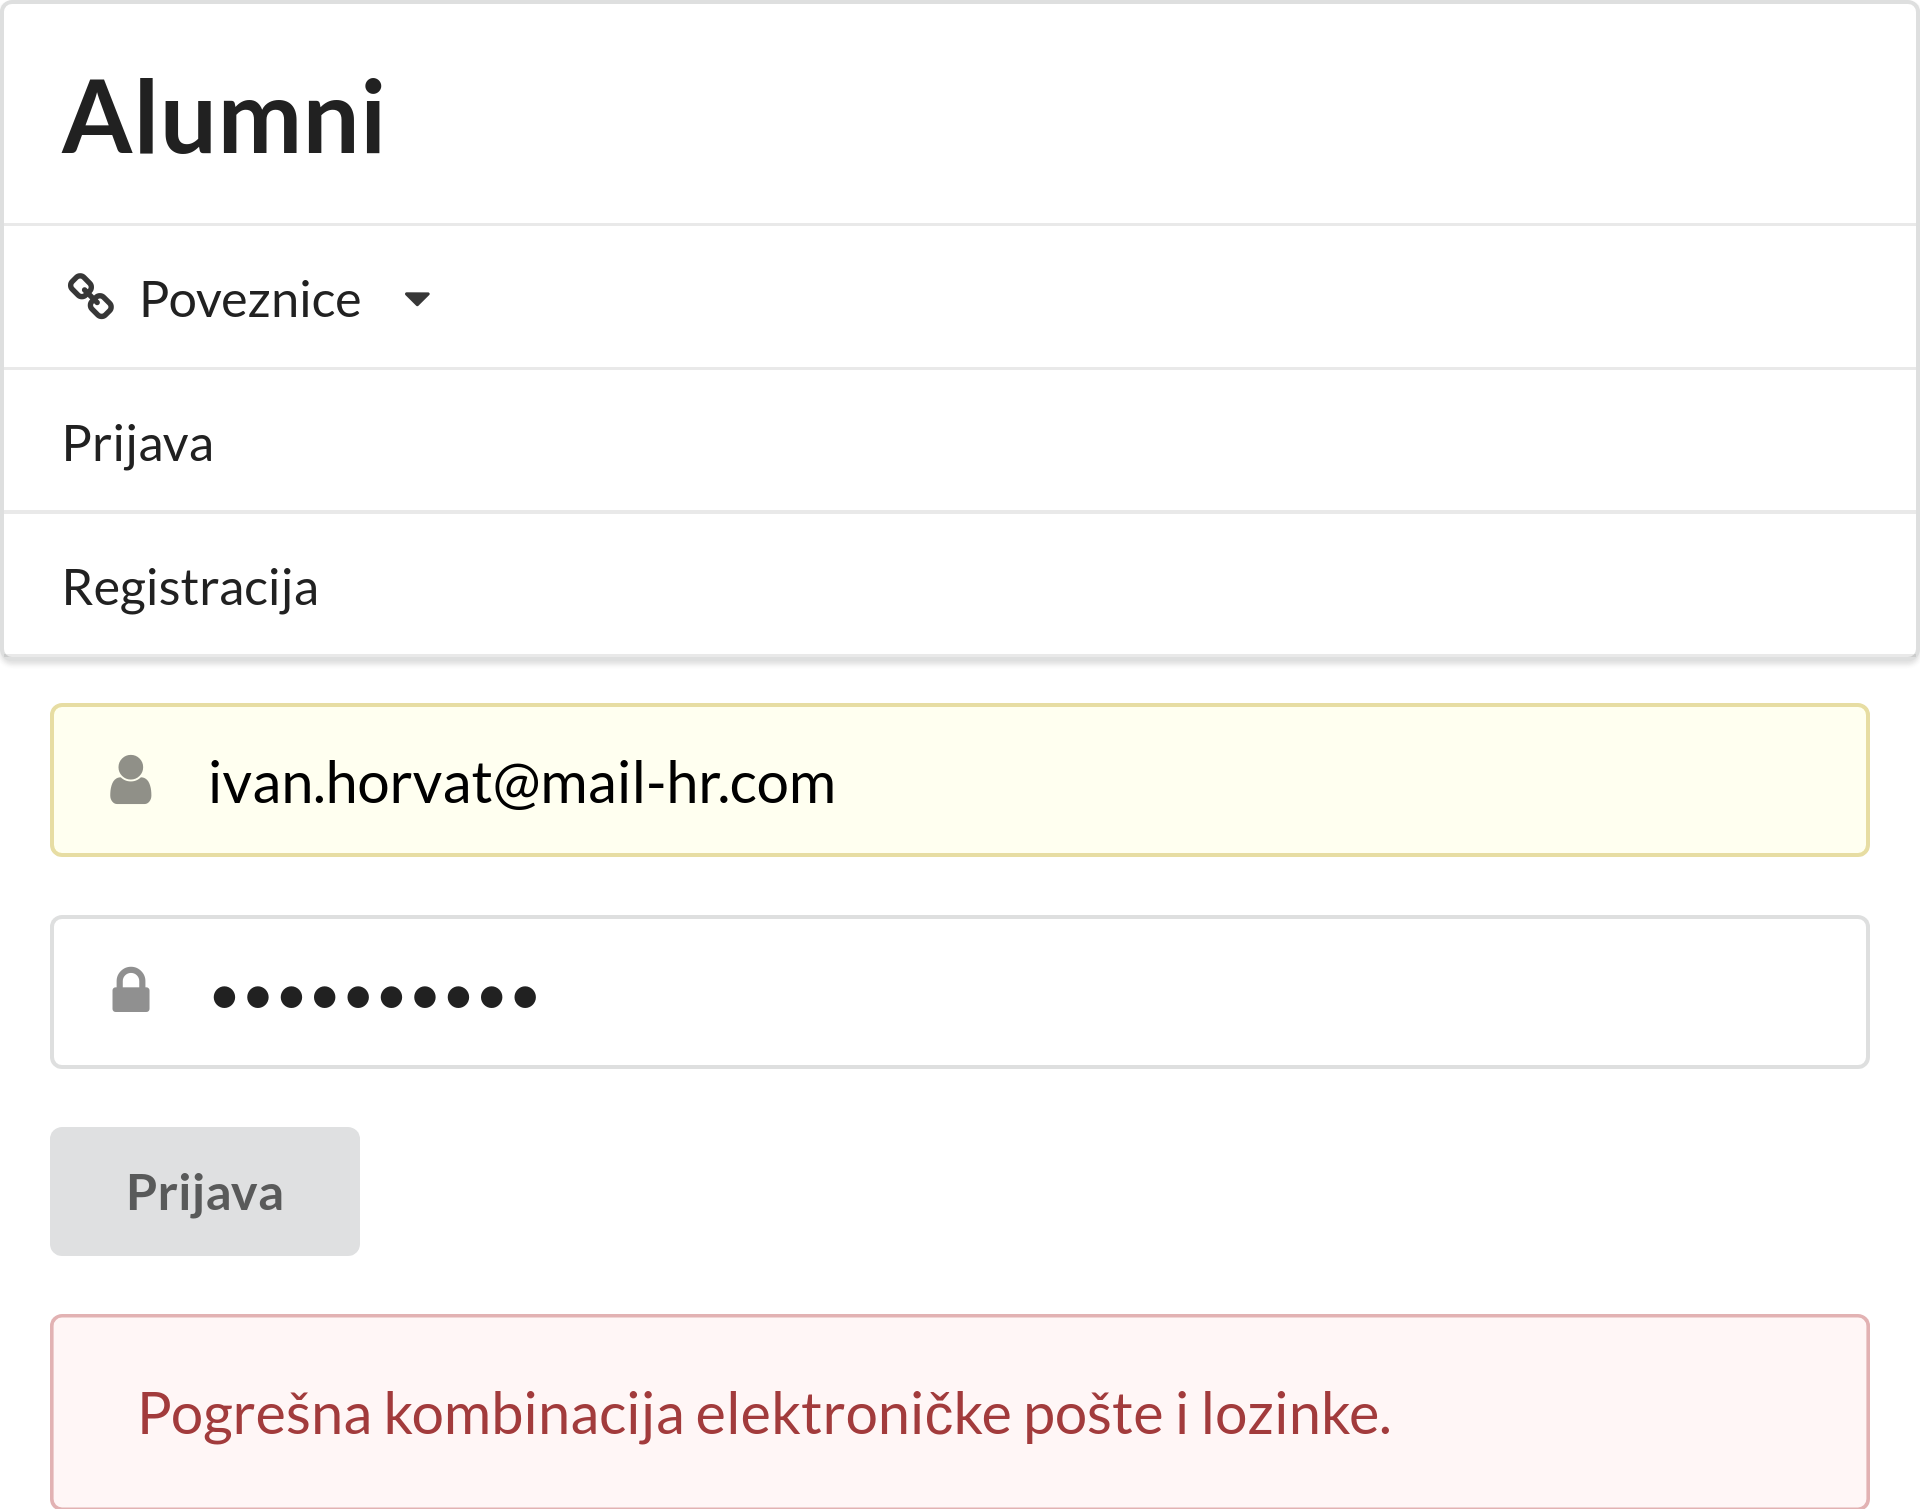
\includegraphics[width=13cm]{slike/prijava.png}
	\caption{Obrazac za prijavu}
	\label{fig:prijava}
\end{figure}

Odabirom "Prijava" na navigacijskoj traci, korisniku se pojavljuje obrazac za prijavu koji se sastoji samo od polja za upis email-a, te polja za upis lozinke. Za oba polja postoji provjera postojanosti, te dodatno za email postoji provjera ispravnosti. Ukoliko se korisnik pokuša prijaviti sa nepostojećim email-om, ili krivo upiše lozinku, prikazati će mu se poruka "Pogrešna kombinacija elektroničke pošte i lozinke". Takva poruka je vrlo popularna u većini aplikacija jer ne otkriva korisniku da li je krivo upisao email ili lozinku, što malo podigne razinu sigurnosti aplikacije.

\subsection{Odjava sa sustava}

\begin{figure}[H]
	\centering
	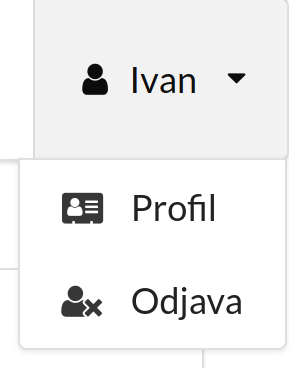
\includegraphics[width=8cm]{slike/odjava.png}
	\caption{Odjava sa sustava}
	\label{fig:odjava}
\end{figure}

Odabirom "Odjava" u padajućem izborniku na desnom kraju trake, korisnik se briše iz trenutne sesije aplikacije i odjavljuje se sa sustava. Time se aplikacija vraća u stanje pregleda koje vidi anoniman korisnik.

\section{Upravljanje korisnicima}
Upravljanje korisnicima je mogućnost koju ima samo administrator, te se sve naredne funkcionalnotsti odnose samo na njega.

\subsection{Pregled svih korisnika}

\begin{figure}[H]
	\centering
	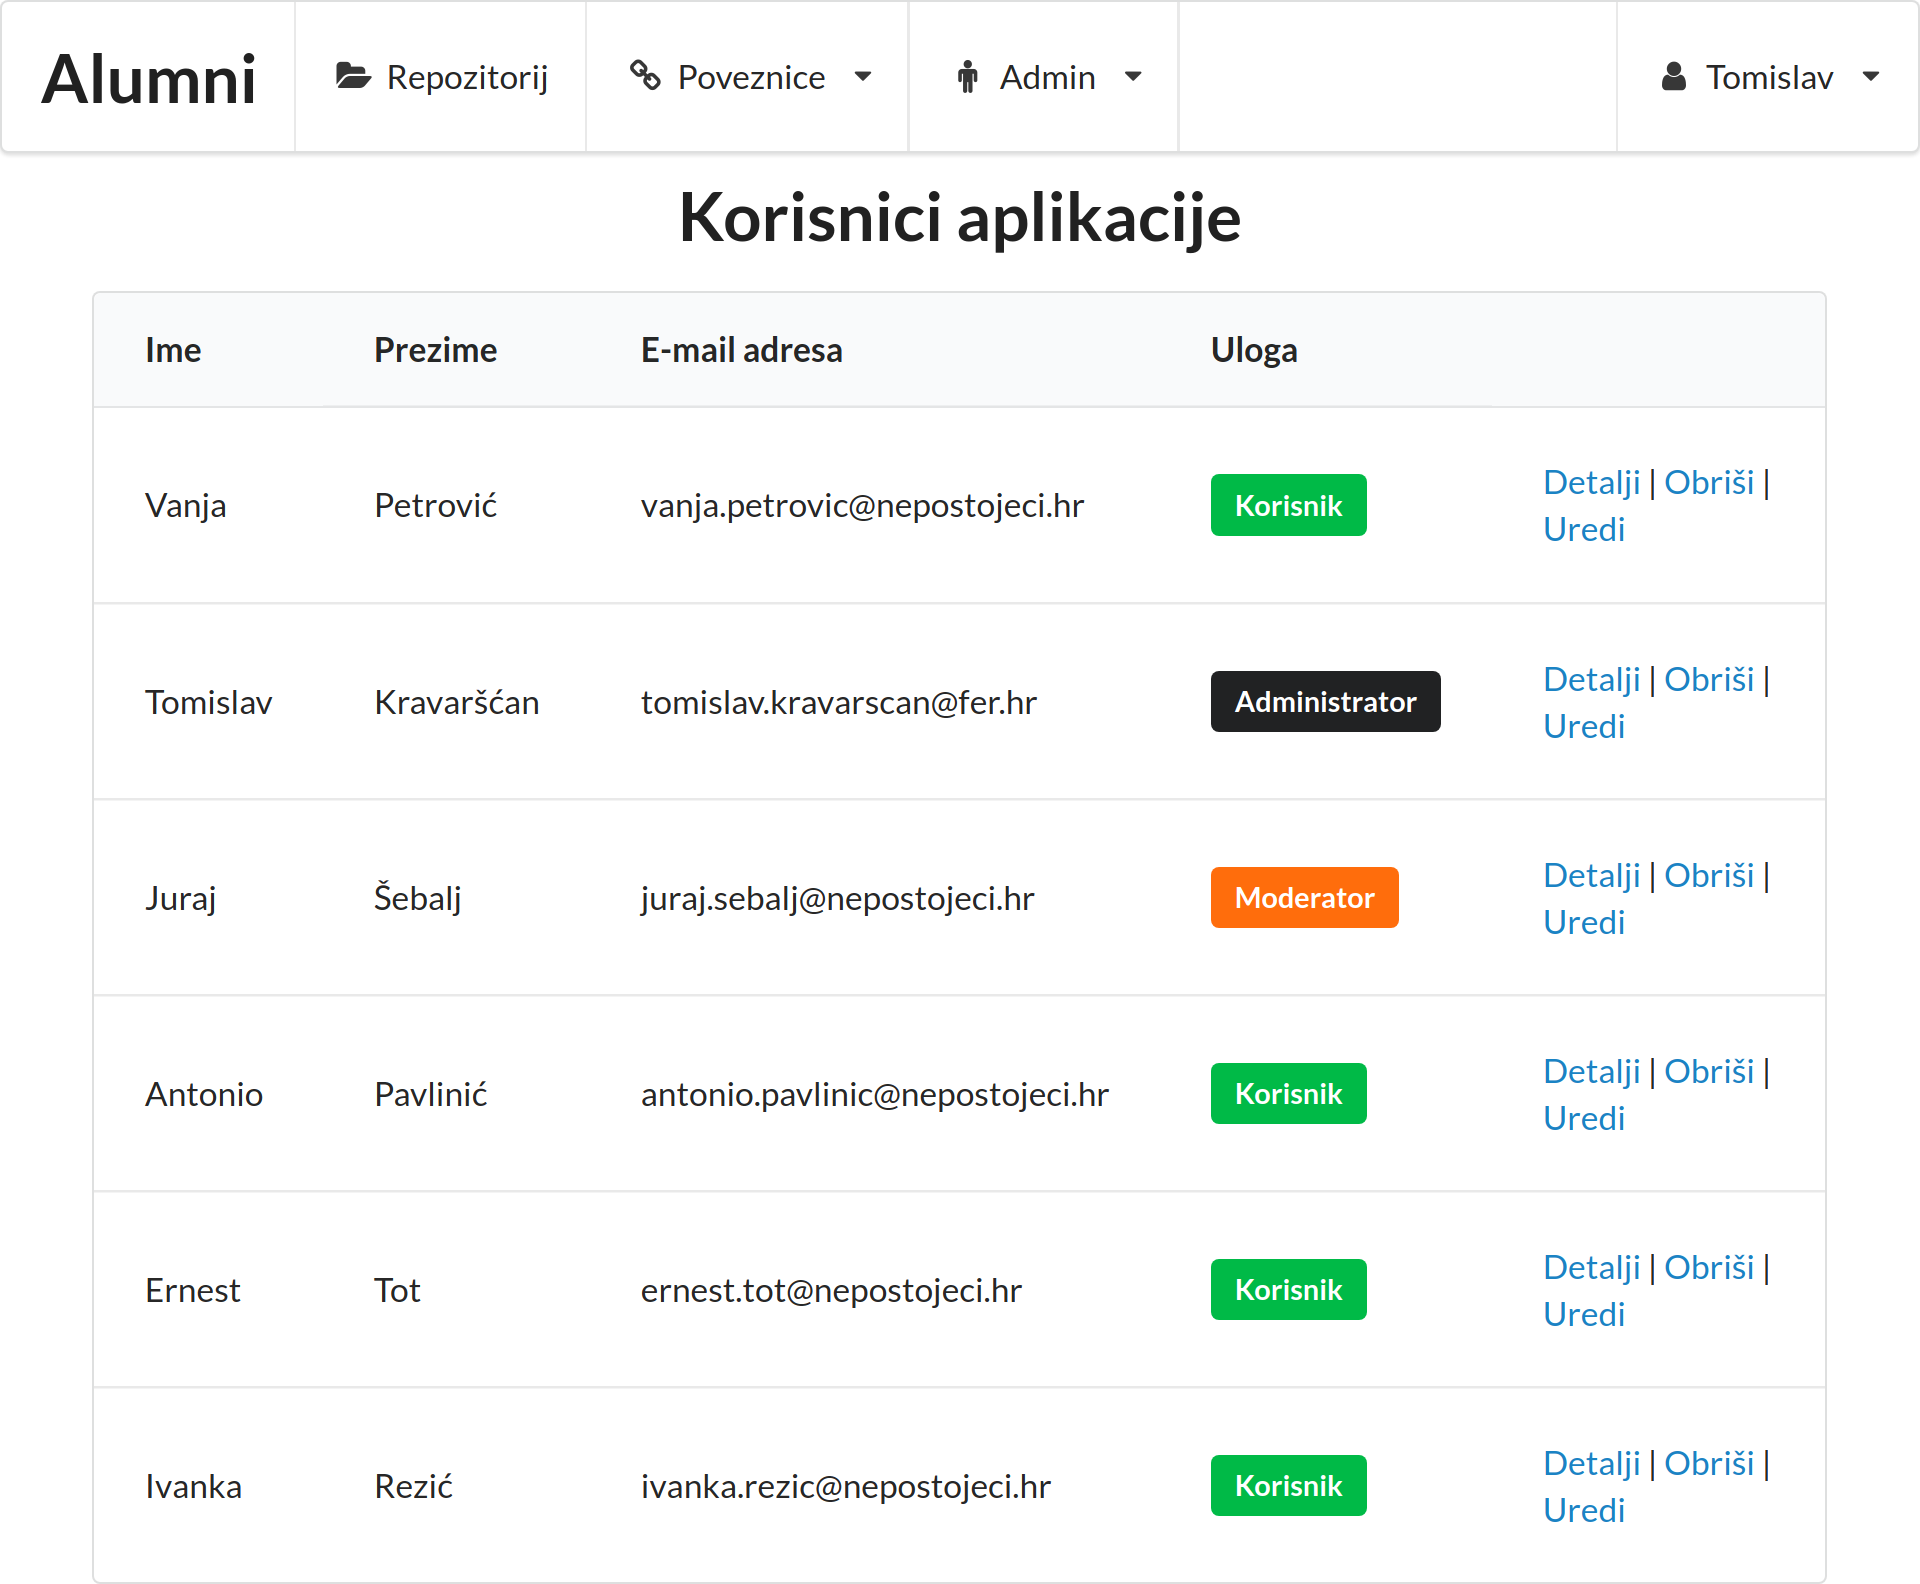
\includegraphics[width=13cm]{slike/korisnici.png}
	\caption{Pregled svih korisnika}
	\label{fig:korisnici}
\end{figure}

Pregled svih korisnika koji se nalaze u aplikaciji ostvaruje se odabirom "Korisnici" u padajućem izborniku "Admin" na navigacijskoj traci. Na tom pregledu su vidljive samo osnovne informacije o korisniku kao što su ime, prezime, email, te uloga korisnika. Osim toga, na desnoj strani zapisa svakog korisnika je moguće odabrati prikaz detalja korisnika, brisanje korisnika te uređivanje korisničkih podataka.

\subsection{Pregled korisničkog računa}

\begin{figure}[H]
	\centering
	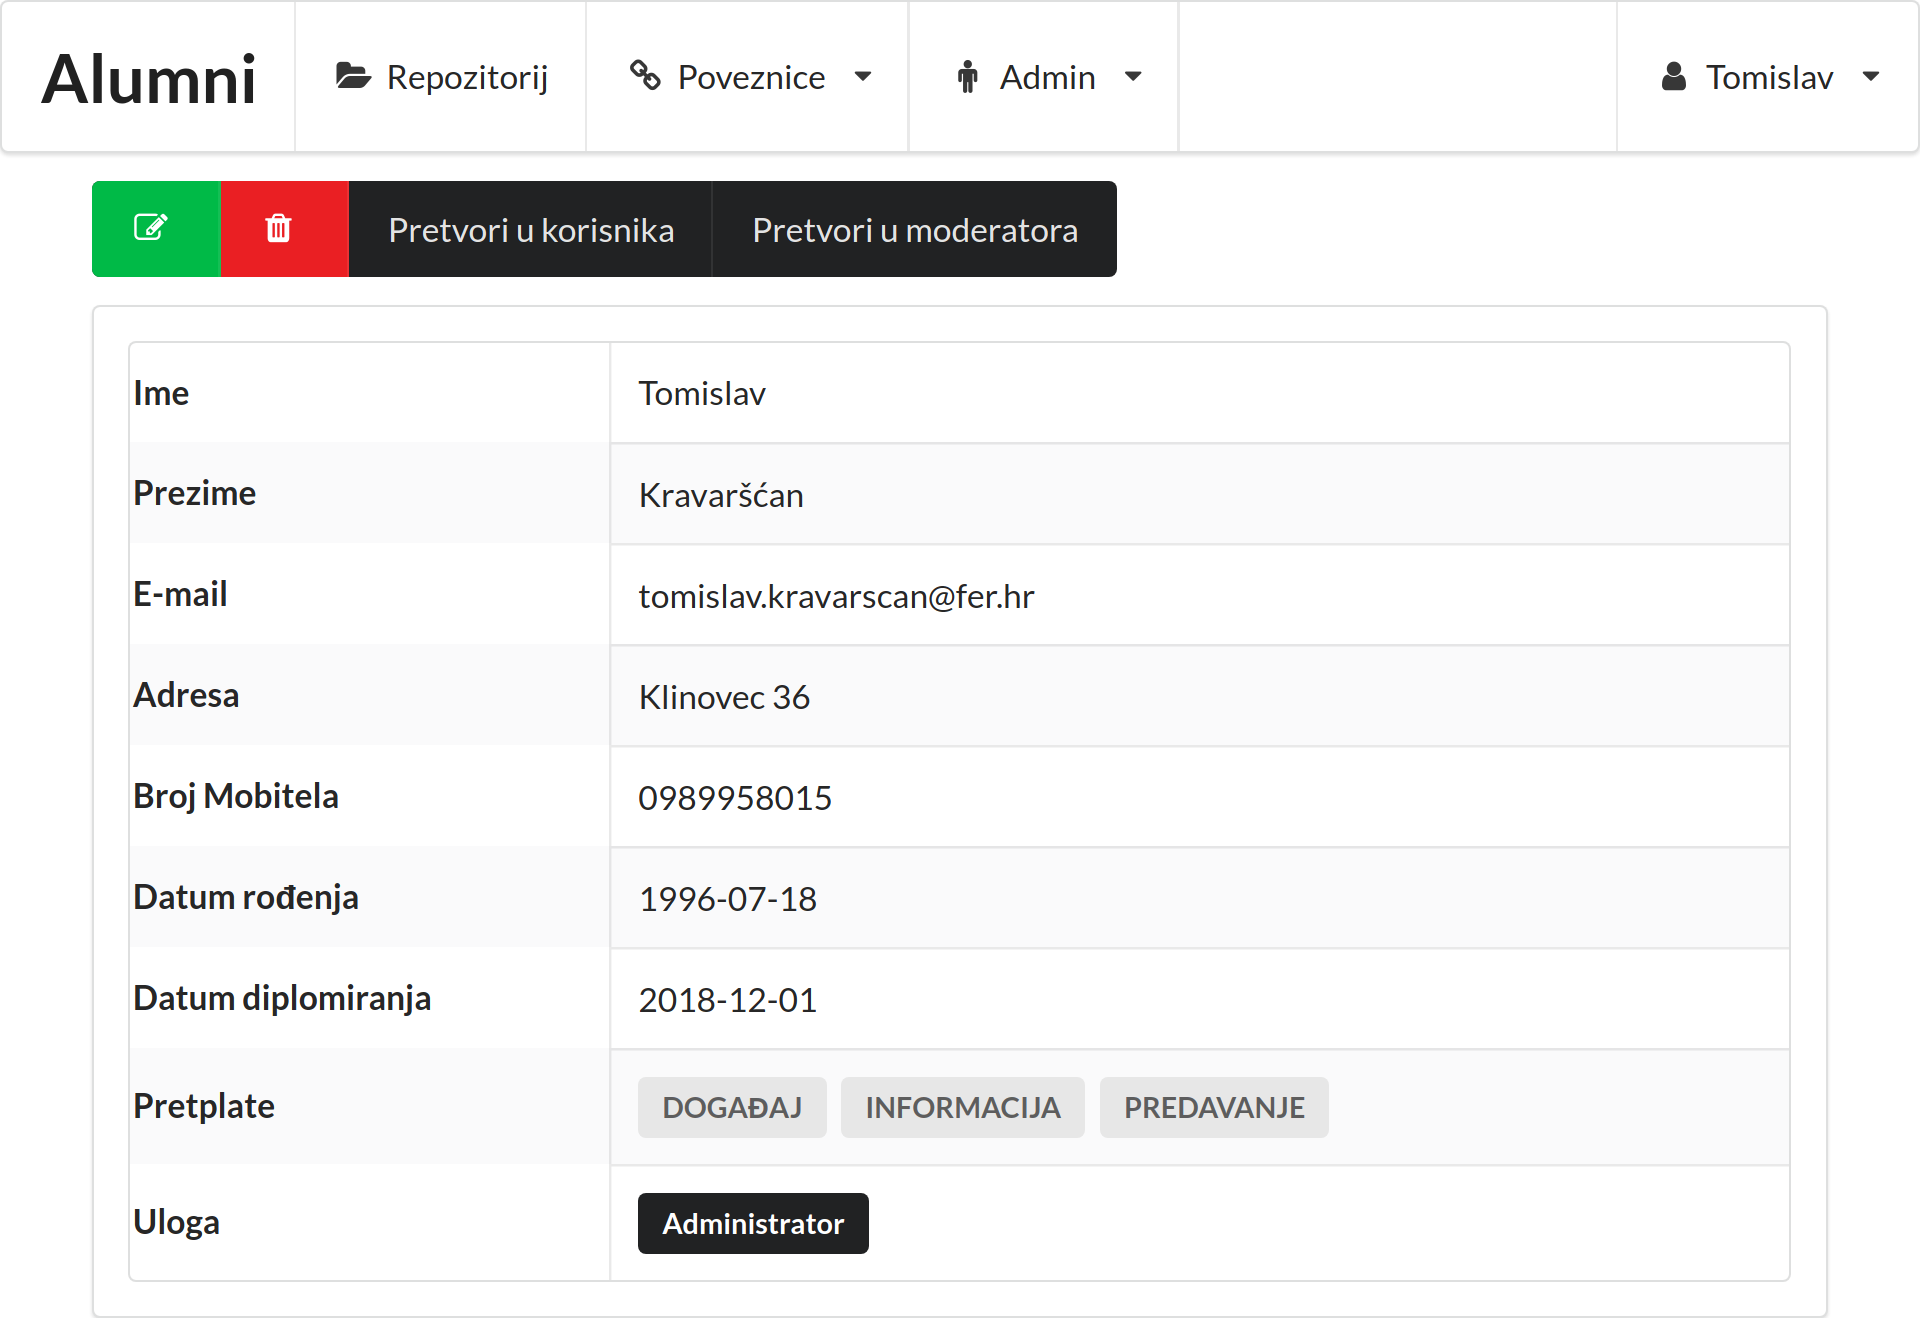
\includegraphics[width=13cm]{slike/profil.png}
	\caption{Korisnički profil}
	\label{fig:profil}
\end{figure}

Administrator može vidjeti sve korisničke račune u sustavu, pa do pregleda korisničkog računa može doći na dva načina: putem padajućeg izbornika u navigacijskoj traci, gdje odabire pregled vlastitog korisničkog računa, te odabirom poveznice detalji na pregledu svih korisnika.

Na pregledu korisničkog računa, imamo sve bitne informacije o korisniku kao što su ime, prezime, email, adresa, broj mobitela, datum rođenja, datum diplomiranja te uloga. Običan korisnik pregledom svog računa može odabrati opciju uređivanja i brisanja pri vrhu stranice za pregled računa, dok administrator ima još opcije promijene uloge korisnika.

\subsection{Uređivanje korisničkog računa}

\begin{figure}[H]
	\centering
	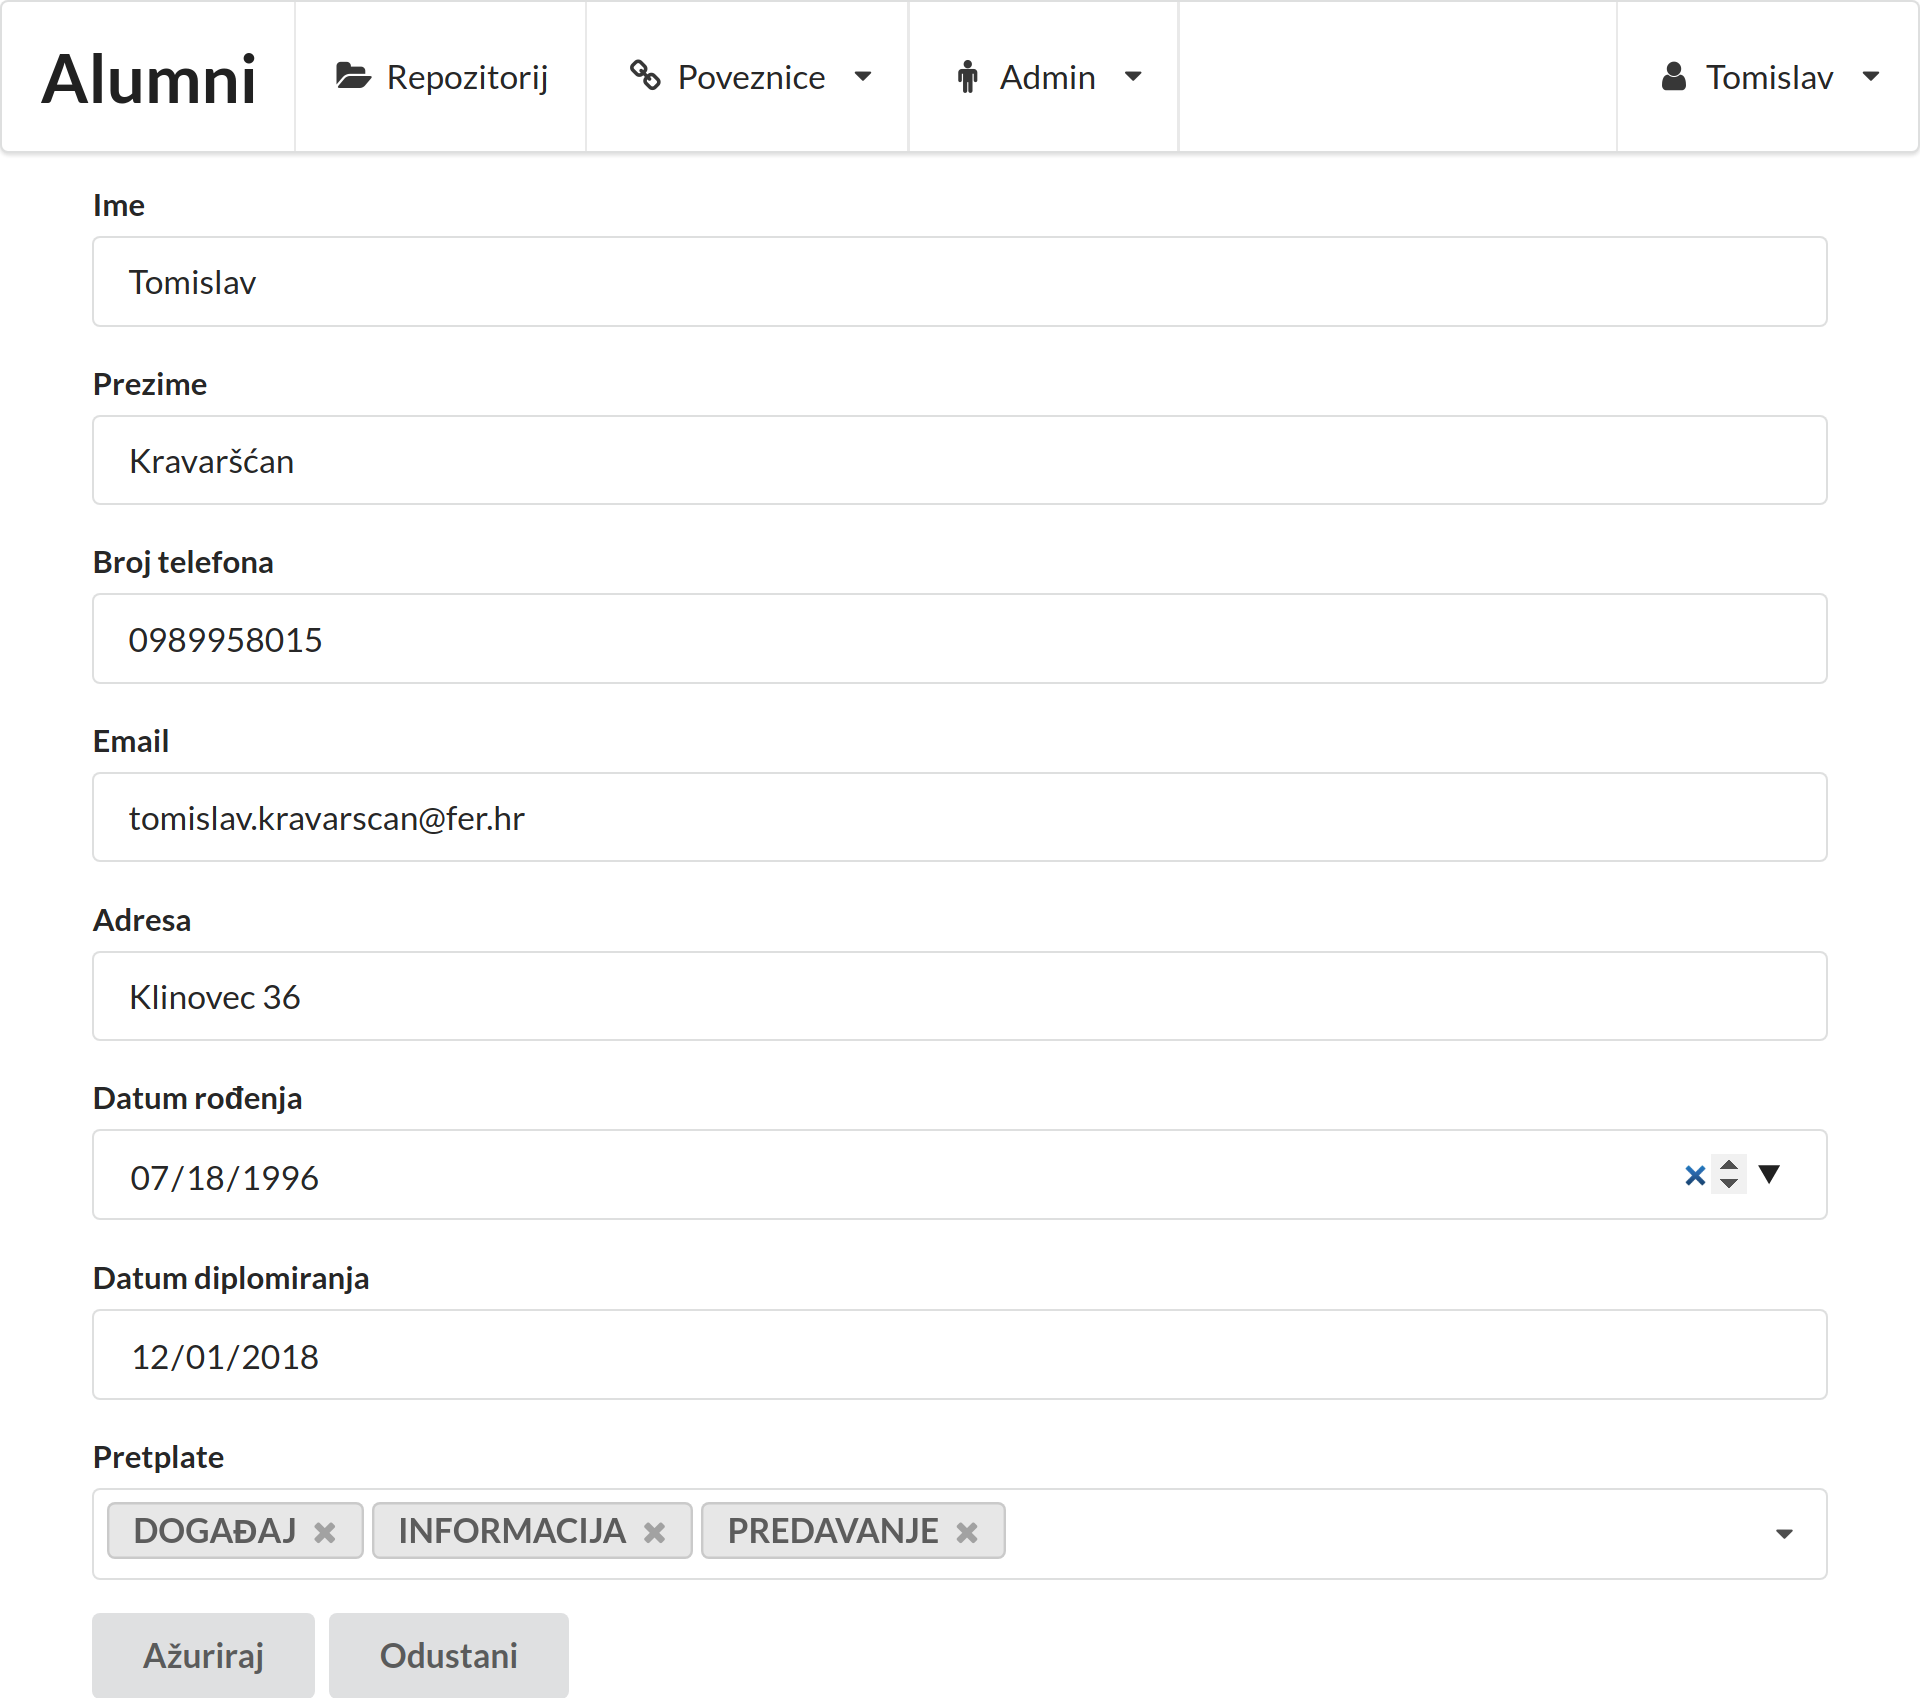
\includegraphics[width=13cm]{slike/uredi-profil.png}
	\caption{Obrazac za uređivanje profila}
	\label{fig:uredi-profil}
\end{figure}

Stranica za uređivanje korisničkog računa je vrlo slična stranici za registraciju, osim što nema upisa lozinke. Korisniku se pojavljuje obrazac gdje su sva polja već ispunjena njegovim podacima. Promijenom bilo kojeg podatka korisnički se račun ažurira i to je odmah vidljivo. Dodatna mogućnost kod uređivanja korisničkog računa je dodavanje pretplata na kategorije postova, o tome će biti više u poglavlju "Sustav pretplata".

\subsection{Promijena uloge korisnika}
Na pregledu korisničkog profila, administrator može promijeniti ulogu korisnika odnosno pretvaranje korisnika u one uloge koje postoje u sustavu, a da ih korisnik trenutno nema. Promijenom uloge korisnik preuzima sve mogućnosti te uloge u sustavu.

\subsection{Brisanje korisničkog računa}
Brisanjem korisničkog računa se iz baze podataka obrišu svi podaci korisnika, te se brišu svi njegovi komentari na postove.

\section{Upravljanje poveznicama}
Poveznice su vrlo bitne za upravljanje bilo kojom udrugom, pa je sustavom za upravljanje poveznicama administratoru koji nije upoznat sa \textit{html} sintaksom i nije u mogućnosti ugraditi poveznice izravno u kod stranice, administratoru omogićeno lagano dodavanje poveznica.

\subsection{Pregled svih poveznica}

\begin{figure}[H]
	\centering
	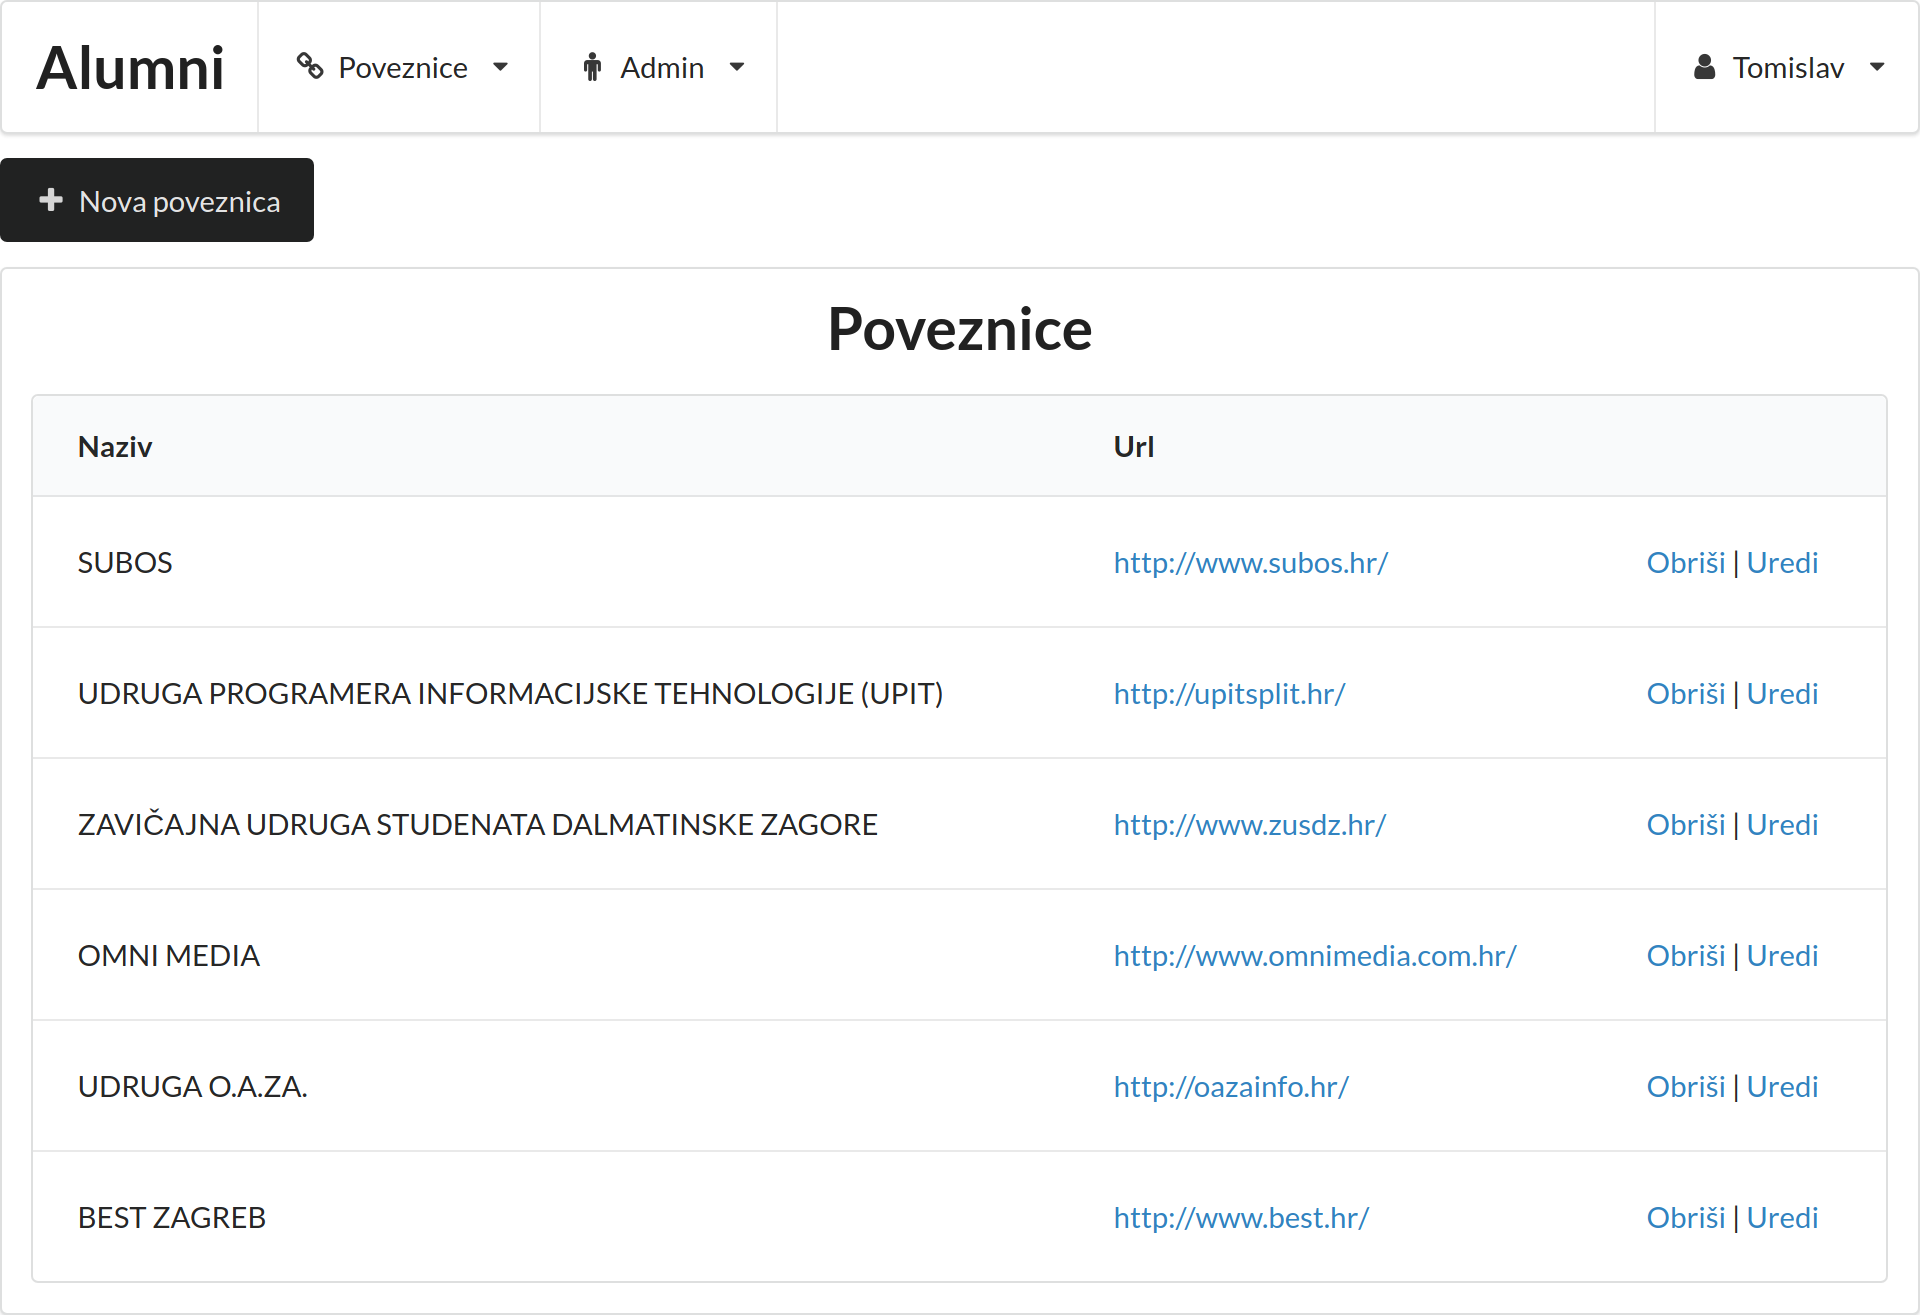
\includegraphics[width=13cm]{slike/poveznice.png}
	\caption{Pregled svih poveznica}
	\label{fig:poveznice}
\end{figure}

Osim što se sve poveznice mogu vidjeti u padajućem izborniku navigacijske trake, za administratora je bitno da ima popis svih poveznica uz dodatne opcije uređivanja i brisanja svake poveznice, slično kao i kod pregleda svih korisnika. Do tog pregleda poveznica dolazi se putem padajućeg izbornika "Admin", odabirom "Stranica poveznica".

\subsection{Dodavanje nove poveznice}

\begin{figure}[H]
	\centering
	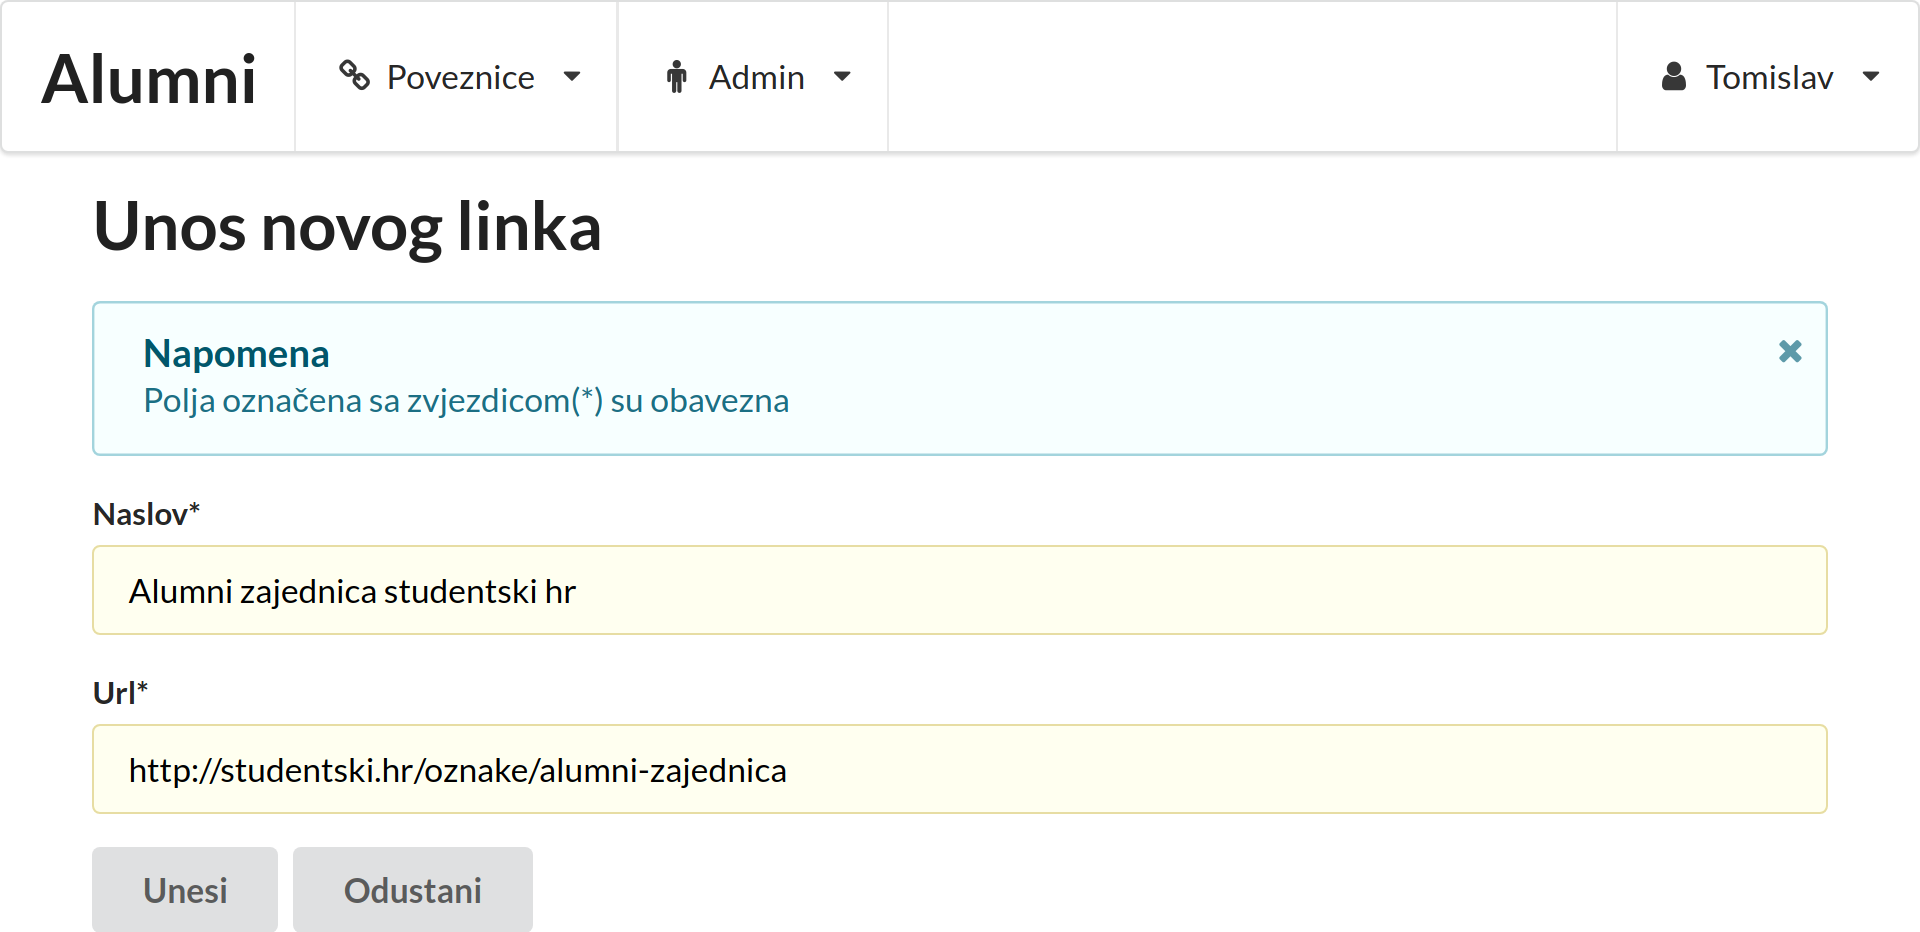
\includegraphics[width=13cm]{slike/nova-poveznica.png}
	\caption{Obrazac za novu poveznicu}
	\label{fig:nova-poveznica}
\end{figure}

Odabirom opcije dodavanja nove poveznice na vrhu pregleda svih poveznica, korisniku se pojavljuje jednostavan obrazac koji ima samo polja naslov i url. Oba polja su obavezna i ne upisivanje bilo kojeg rezultira pogreškom, dodatno, url mora biti ispravnog formata i započinjati sa oznakom protokola.

\subsection{Uređivanje poveznice}
Odabirom opcije uređivanja poveznice na desnoj strani zapisa svake poveznice prikazuje se isti obrazac kao i kod stvaranja poveznice, uz to da su podaci o poveznici već upisani. 

\subsection{Brisanje poveznice}
Odabirom brisanja poveznice, poveznica se uklanja iz sustava.

\section{Upravljanje kategorijama}
Svaki post u sustavu mora imati određenu kategoriju. Zbog olakšanog proširivanja funkcionalnosti aplikacije administratoru je omogućeno dinamičko stvaranje novih kategorija postova. 

\subsection{Pregled svih kategorija}

\begin{figure}[H]
	\centering
	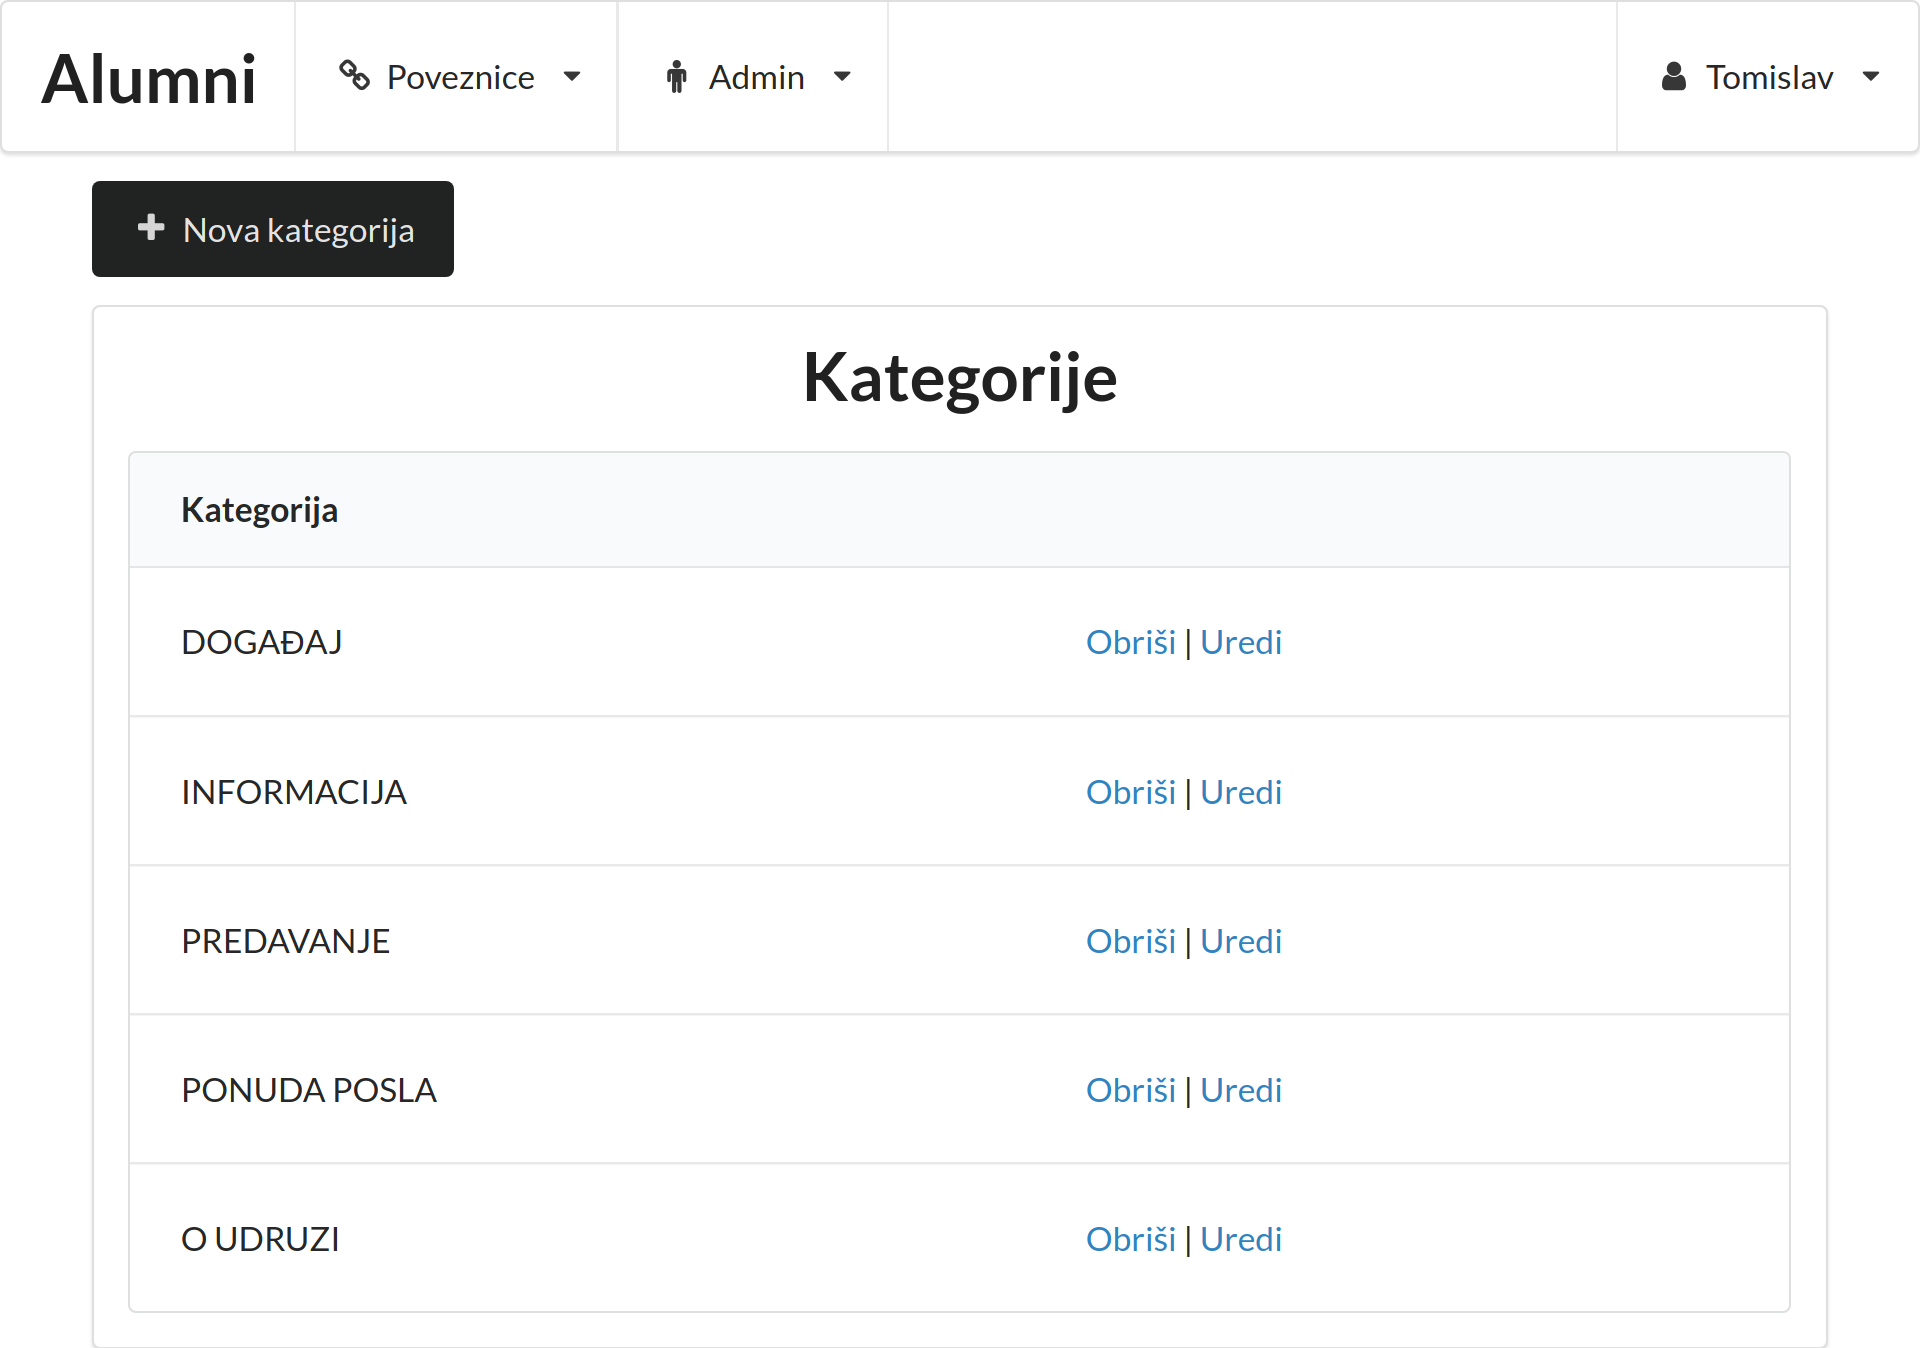
\includegraphics[width=13cm]{slike/kategorije.png}
	\caption{Pregled svih kategorija}
	\label{fig:kategorije}
\end{figure}

Do pregleda svih kategorija dolazi se putem padajućeg izbornika "Admin" u navigacijskoj traci, odabirom na "Kategorije". Za svaku kategoriju prikazan je samo njen naziv, te postoje mogućnosti brisanja i uređivanja. Osim toga, na vrhu stranice je opcija dodavanja nove kategorije.

\subsection{Dodavanje nove kategorije}

\begin{figure}[H]
	\centering
	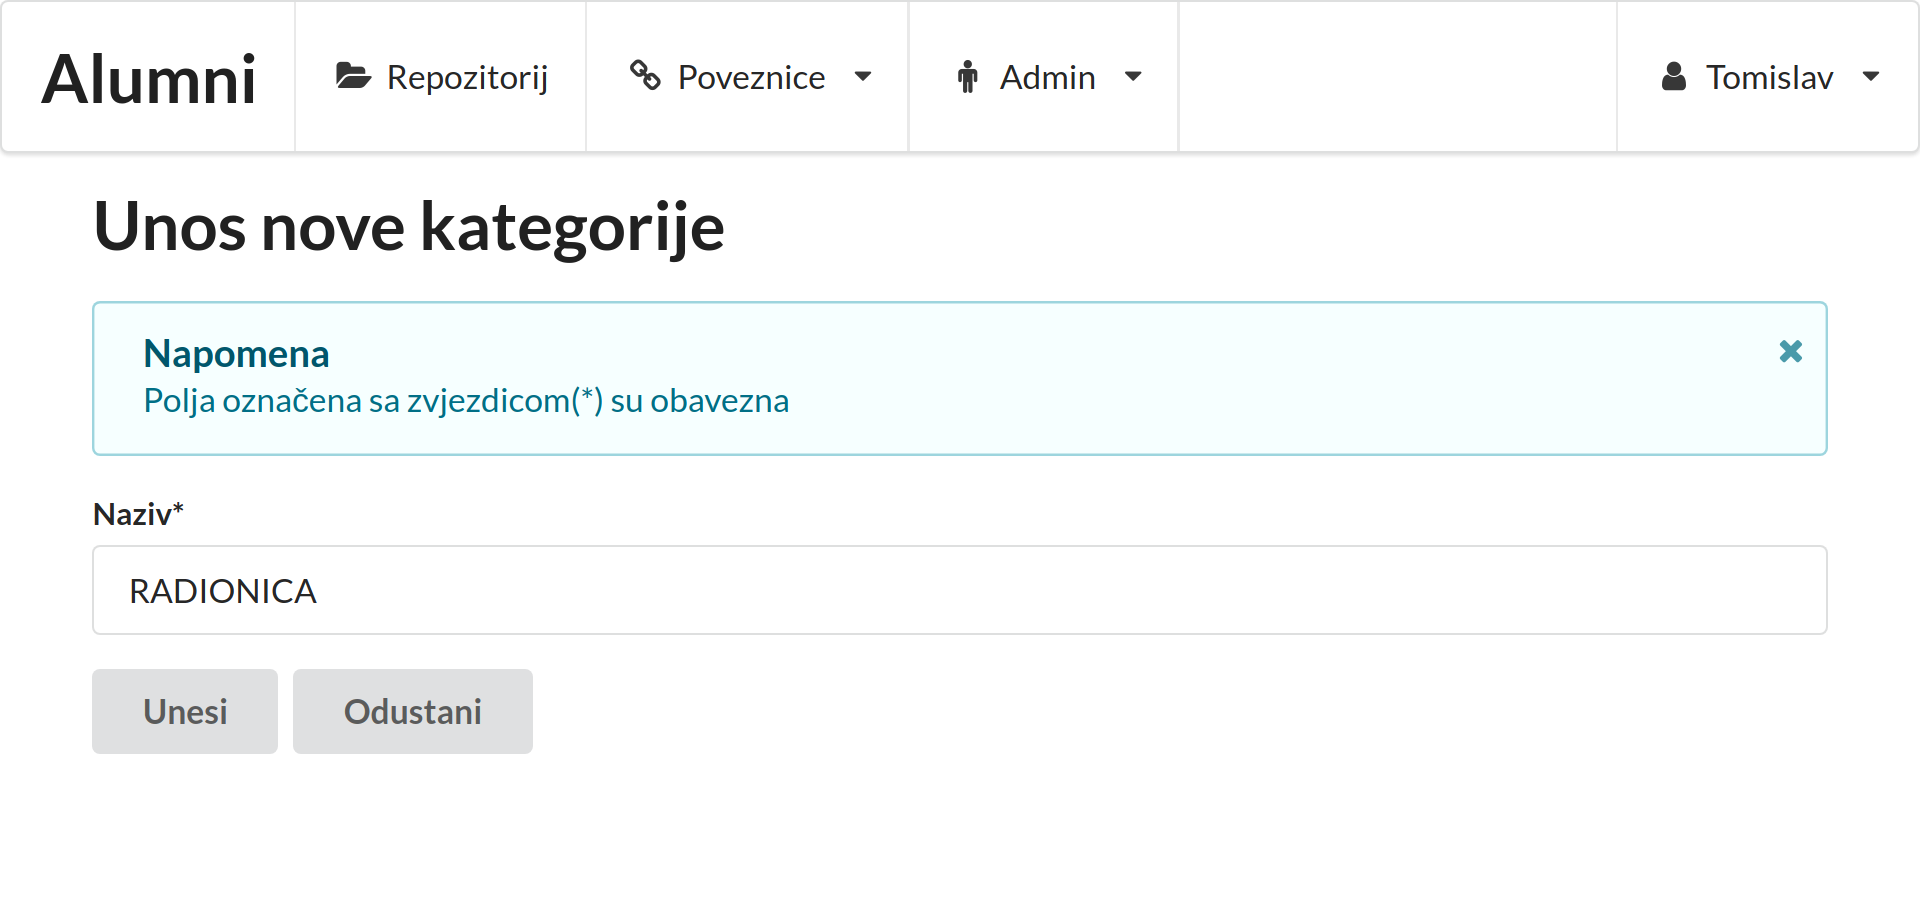
\includegraphics[width=13cm]{slike/nova-kategorija.png}
	\caption{Obrazac za novu kategoriju}
	\label{fig:nova-kategorija}
\end{figure}

Dodavanje nove kategorije je vrlo jednostavno i obrazac ima samo jedno polje, naslov kategorije. To polje naravno ne smije biti prazno.

\subsection{Uređivanje kategorije}
Kategorija se može urediti, i to se obavlja na isti način kao i kod stvaranja.

\subsection{Brisanje kategorije}
Kod pokušaja brisanja kategorije, ako postoje postovi koji su te kategorije, aplikacija će nam zabraniti taj pokušaj. Prvo je potrebno obrisati sve postove s tom kategorijom, ili svim takvim postovima ukloniti kategoriju koju želimo obrisati.

\section{Upravljanje postovima}
Upravljane postovima je gotovo najbitnija funkcionalnost kod programske podrške za neku zajednicu. Vrlo je bitno na pregledan način korisnicima prikazati sve relevantne novosti.

\subsection{Pregled svih postova}

\begin{figure}[H]
	\centering
	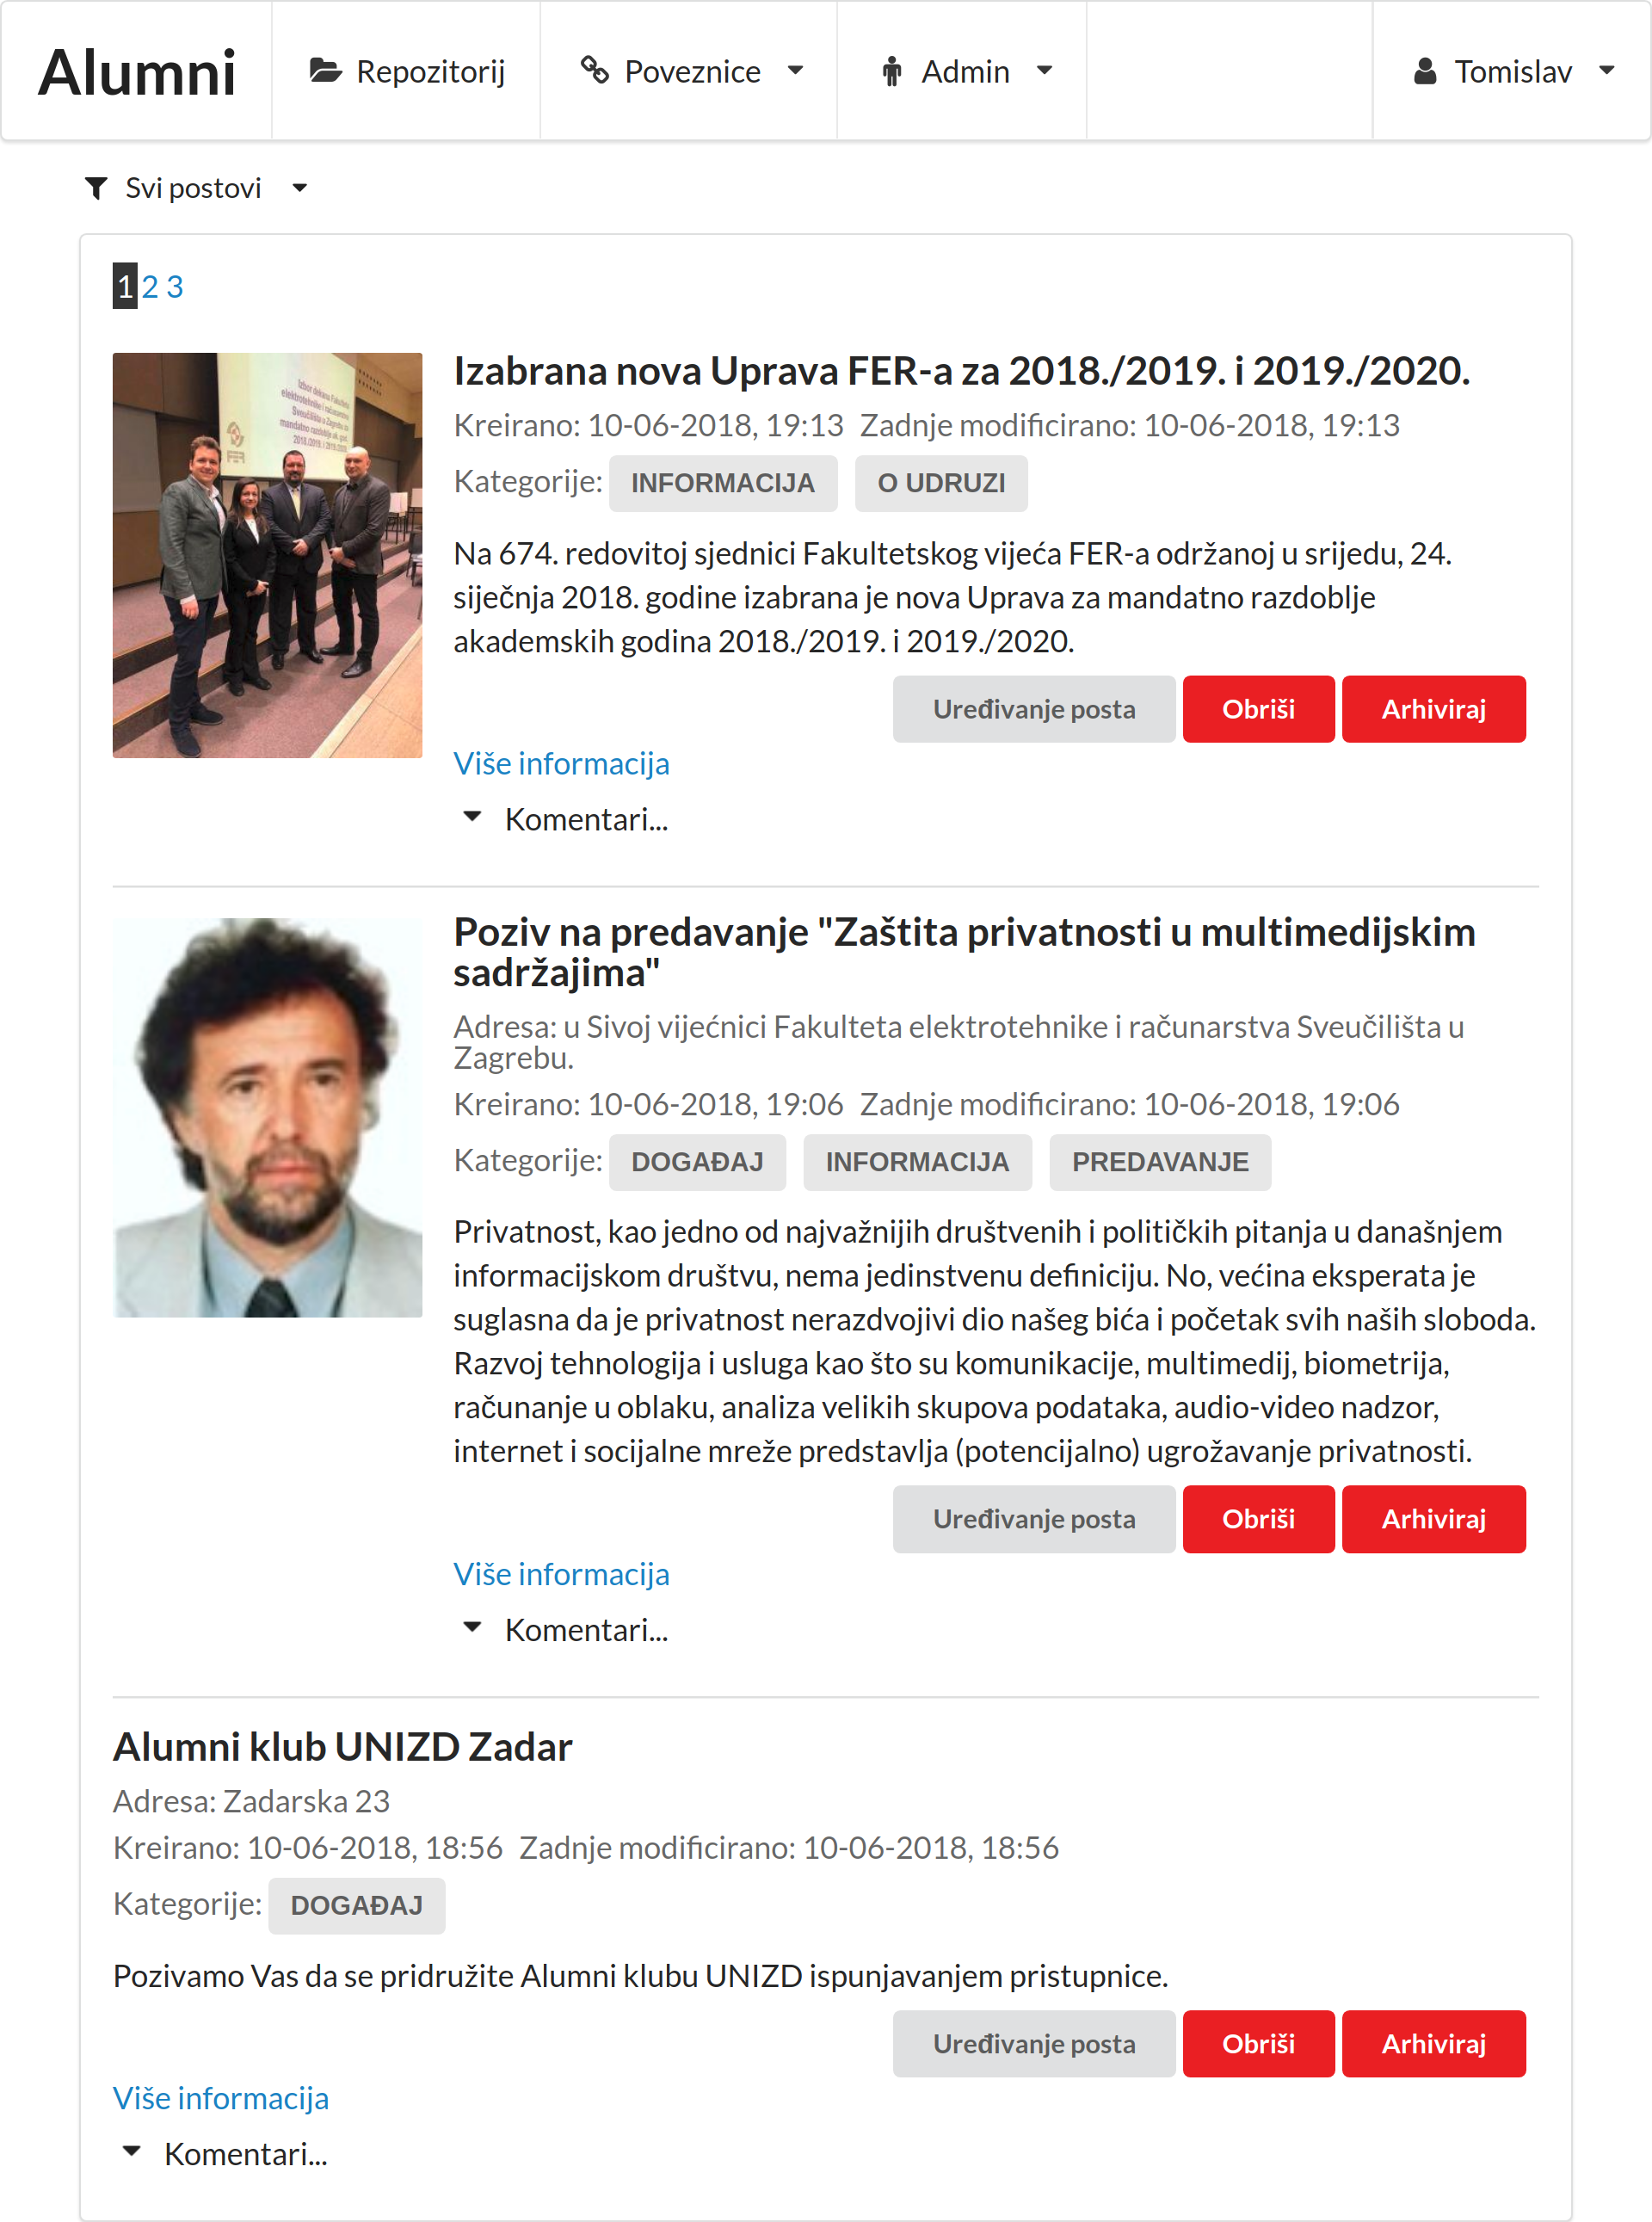
\includegraphics[width=13cm]{slike/postovi.png}
	\caption{Početna stranica - pregled svih postova}
	\label{fig:postovi}
\end{figure}

Svi postovi se nalaze na početnoj stranici aplikacije, do koje se i u svakom dijelu aplikacije može doći odabirom "Alumni" u navigacijskoj traci. Na početnoj se stranici ne nalaze sve informacije vezane za određene postove. Početna je stranica zamišljena kao sažetak postova, dok se puni opis svakog posta nalazi na njegovoj zasebnoj stranici. Na pregledu svih postova vidimo naslov posta, adresu (lokaciju odrđavanja ako je događaj), datum izrade posta, datum zadnjeg uređivanja posta, kategorije, kratki opis. Dodatno, odabirom na "Komentari..." pojavljuje se padaući element sa svim komentarima posta, na kojem korisnik može i komentirati taj post ako je prijavljen. Uz to, administrator na pregledu svih postova ima mogućnost uređivanja, brisanja i arhiviranja svih postova, te brisanja komentara.

Kako nebi bilo previše postova na stranici, postoji sustav straničenja.

\subsection{Filtriranje postova}

\begin{figure}[H]
	\centering
	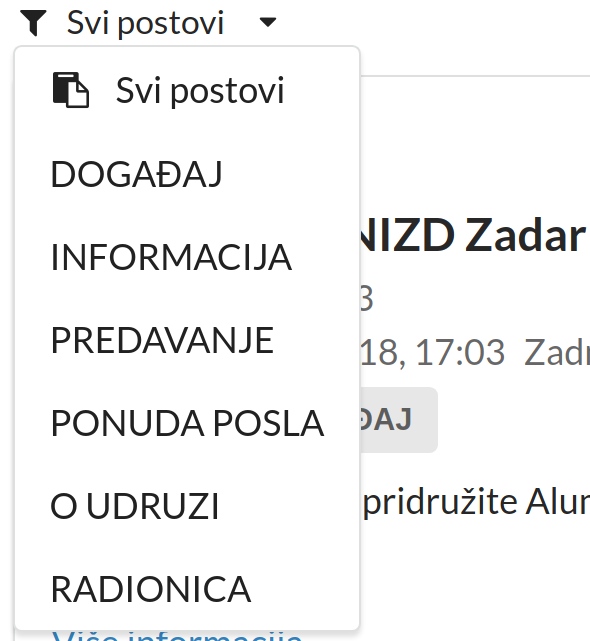
\includegraphics[width=13cm]{slike/filter.png}
	\caption{Padajući izbornik za filtriranje postova}
	\label{fig:filter}
\end{figure}

Postovi mogu biti različitih kategorija, a korisniku sustava često neće biti bitne sve te kategorije. Zbog toga je korisniku omogućeno filtriranje postova po kategorijama putem padajućeg izbornika na vrhu stranice svih postova. Tekst padajućeg izbornika se dinamički mijenja, te se ovisno o tome koja je kategorija izabrana za filtriranje tekst postavi na naziv te kategorije. Osim filtriranja pomoću tog izbornika, filtriranje se može obaviti i odabirom na oznaku kategorije na svakom postu.

\subsection{Pregled posta}

\begin{figure}[H]
	\centering
	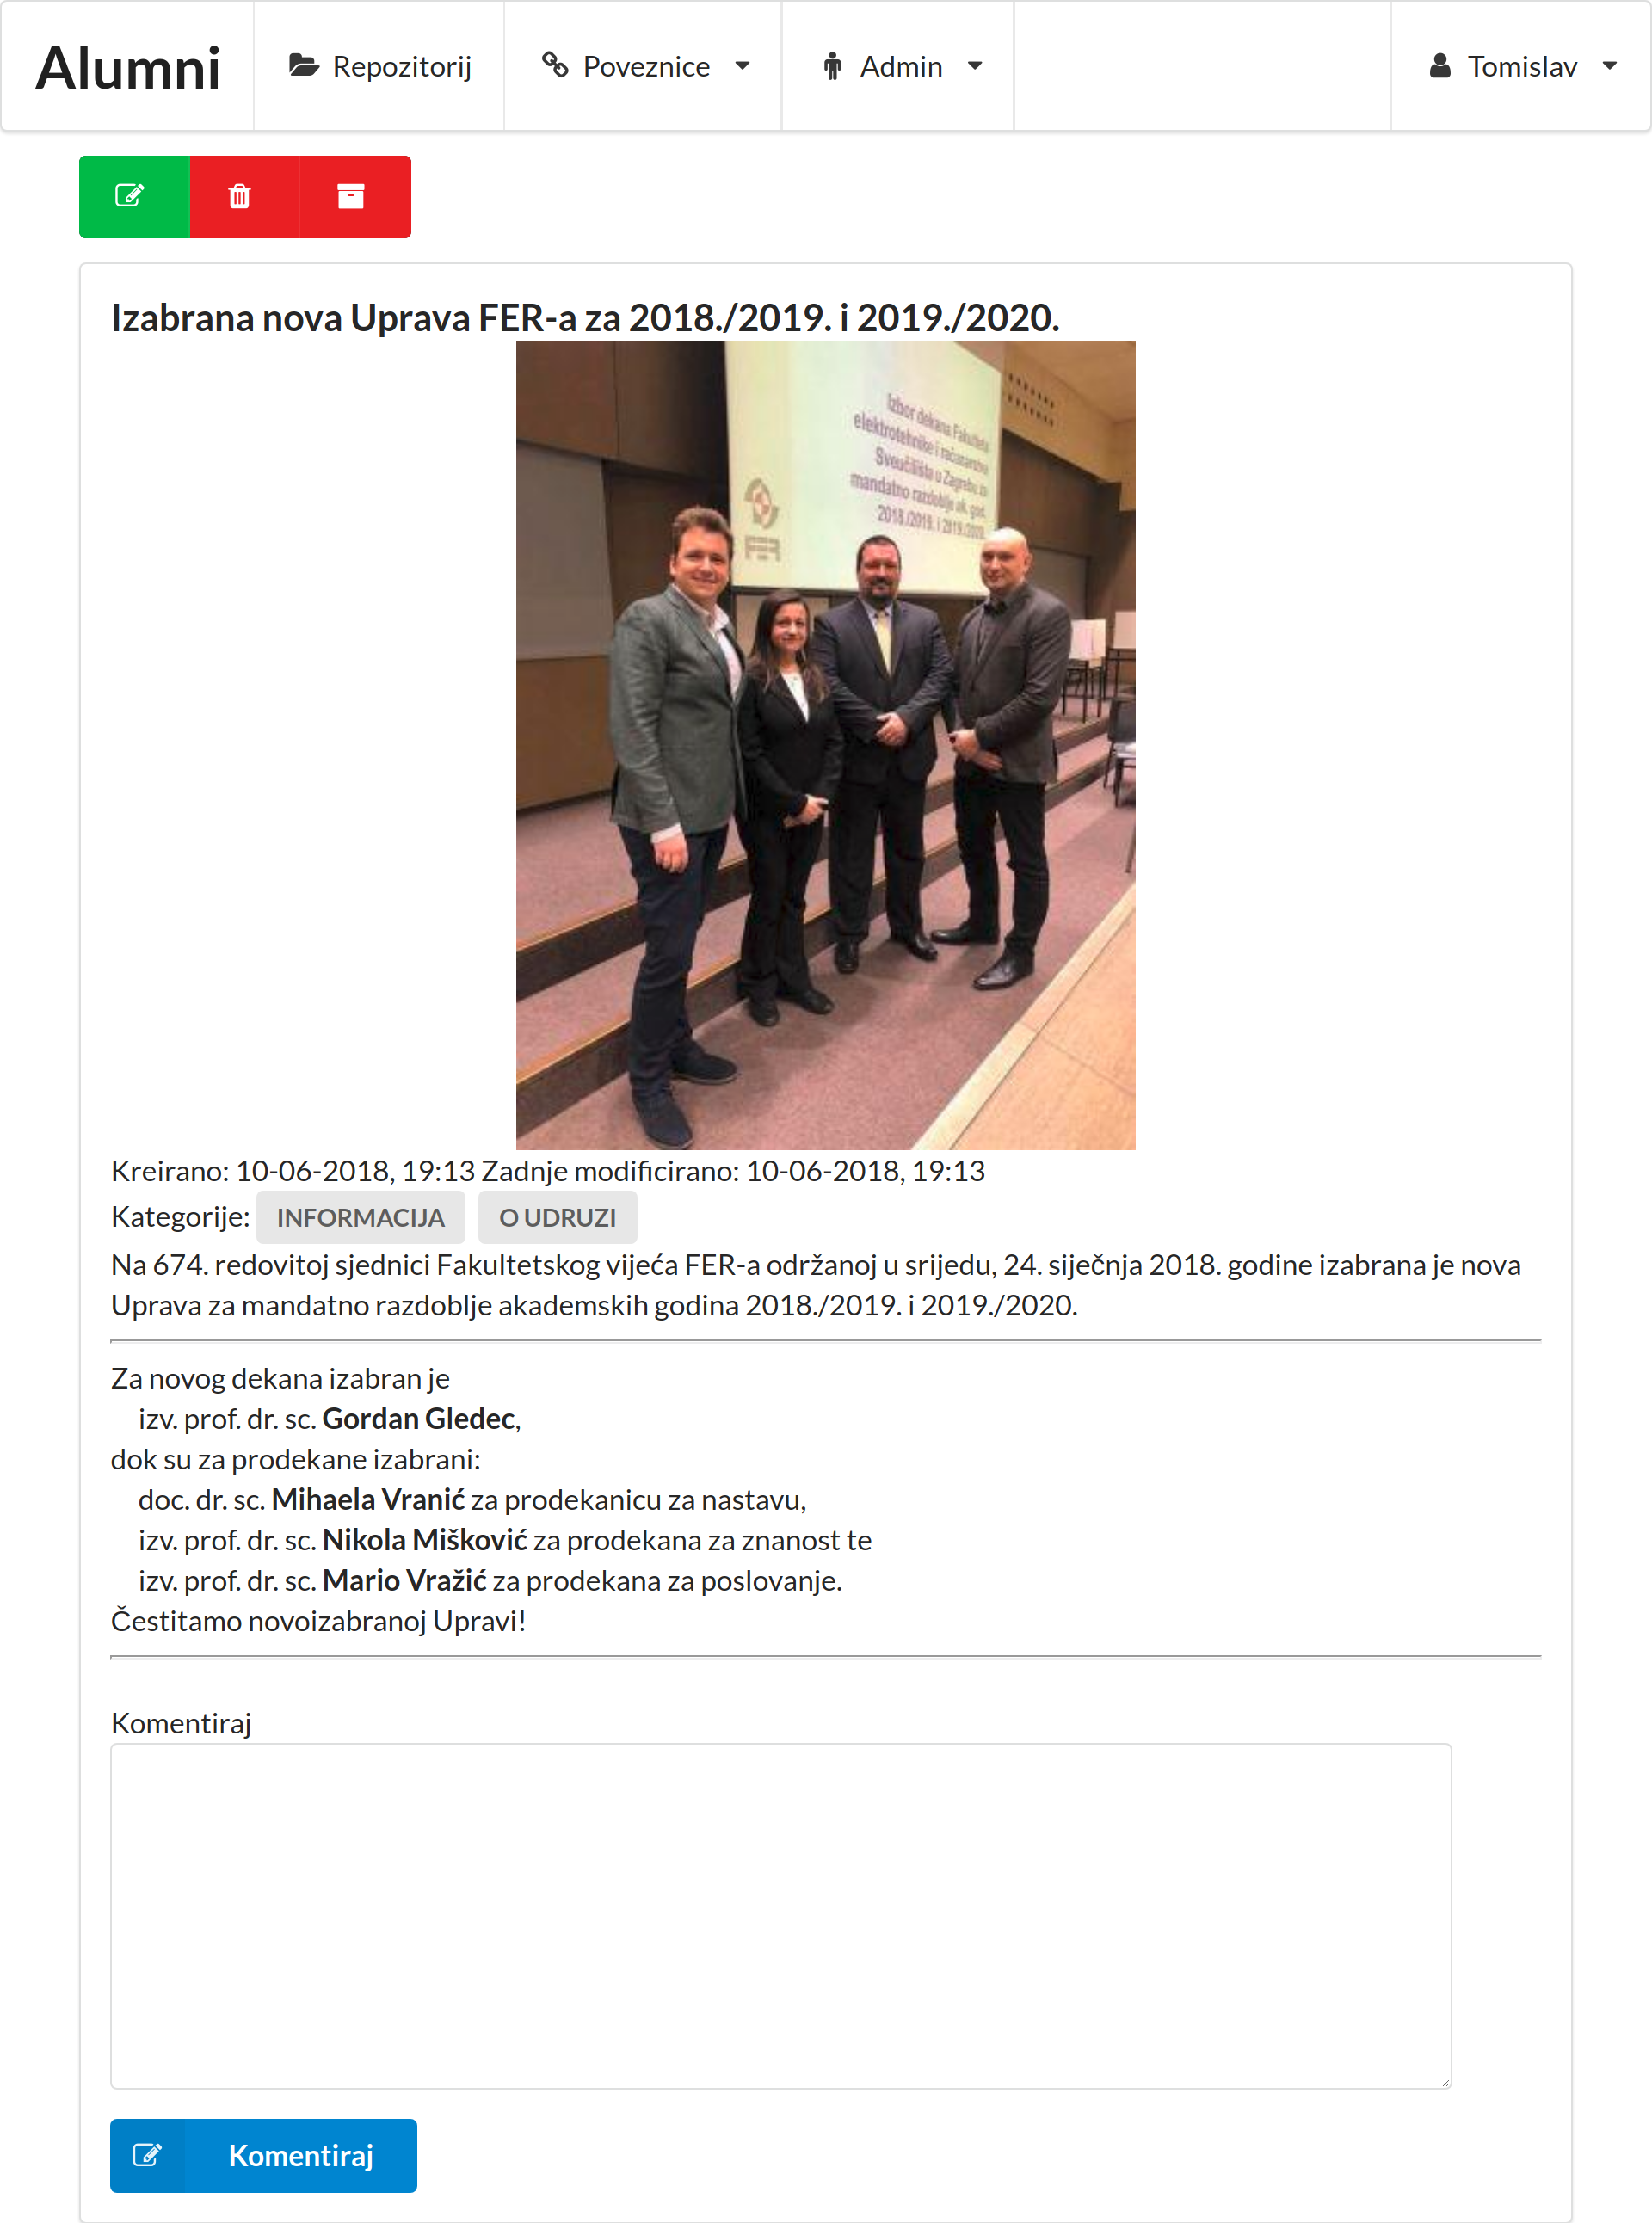
\includegraphics[width=13cm]{slike/post.png}
	\caption{Pregled posta}
	\label{fig:post}
\end{figure}

Odabirom poveznice "Više informacija" ili odabirom naslova posta na stranici pregleda svih postova, dolazi se do stranice za pregled određenog posta gdje se nalazi sve što postoji i na pregledu svih postova, uz dodatan dio gdje se nalazi dugi opis posta.

Također, pri vrhu stranice nalaze se administratorske opcije uređivanja, brisanja te arhiviranja posta.
 
\subsection{Dodavanje novog posta}

\begin{figure}[H]
	\centering
	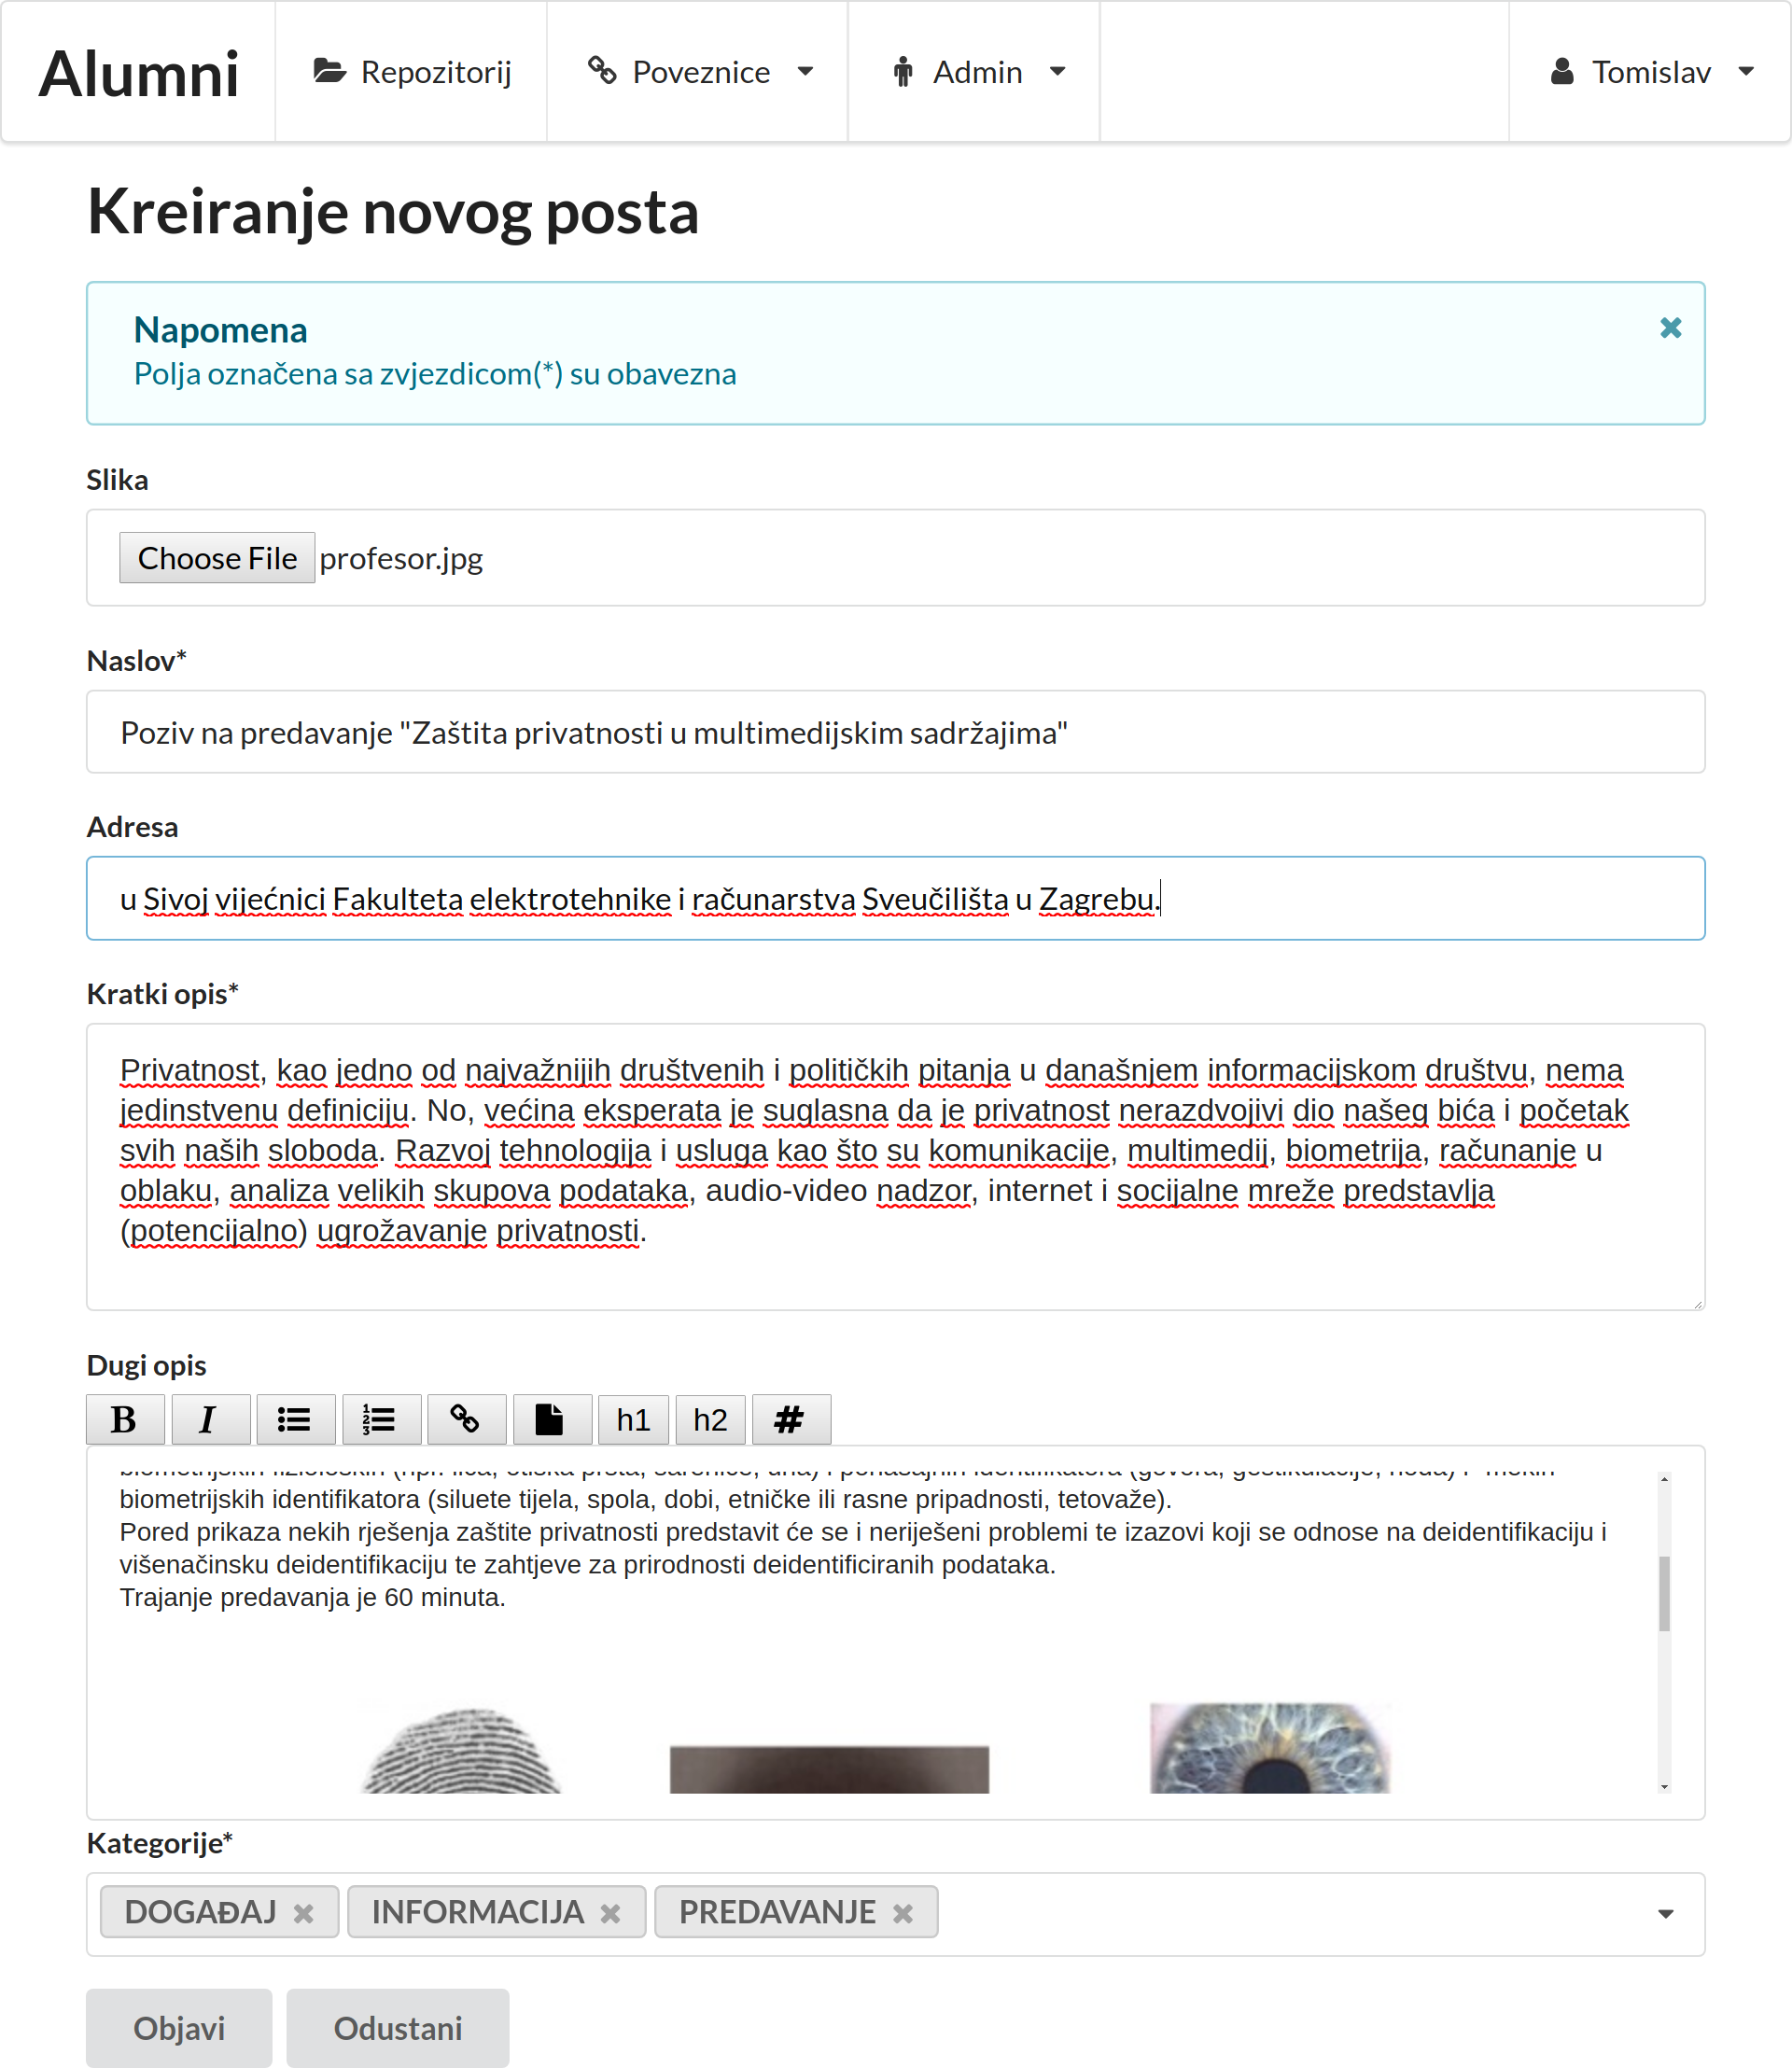
\includegraphics[width=13cm]{slike/novi-post.png}
	\caption{Obrazac za dodavanje novog posta}
	\label{fig:novi-post}
\end{figure}

Do obrasca za dodavanje novog posta dolazi se odabirom opcije "Novi post" u padajućem izborniku "Admin". Dodavanje novog posta zahtijeva upis naslova, kratkog opisa te odabira kategorija postova. Dok su neobavezna polja adresa(lokacija održavanja ako je događaj, dvorana ako je predavanje) i dugi opis posta. Dodavanje dugog opisa posta ostvareno je funkcionalnim uređivačem teksta, zbog administratora koji možda nisu upoznati sa \textit{html} sintaksom. Kao opcije za uređivanje omogućeno je podebljanje teksta, ukošavanje teksta, izrada neporedane liste, izrada poredane, brojevima označene liste, ubacivanje poveznice, ubacivanje slike, izrada velikog naslova, izrada naslova srednje veličine, te prikaz teksta u \textit{html} formatu za naprednije korisnike koji žele dodatno uljepšati tekst opcijama koje nisu ponuđene.

\subsection{Uređivanje posta}
Uređivanje posta je ostvareno tako da bude gotovo identično stvaranju novog posta, uz već upisana polja s postojećim podacima.

\subsection{Brisanje posta}
Brisanjem posta brišu se i svi komentari na taj post, a ostvarivo je preko stranice za pregled svih postova ili preko stranice za dotični post koji želimo obrisati.

\subsection{Arhiviranje posta}
Arhiviranje posta je vrlo bitno jer postovi nakon nekog vremena postaju beznačajni, npr. nakon odvijanja događaja o kojem je bio taj post. Ali svejedno ga ne želimo iz nekog razloga obrisati iz sustava jer možda sadrži neku bitnu informaciju, ili čisto radi statistike. Zbog toga postoji funkcionalnost arhiviranja posta koju odrađuje administrator odabirom opcije arhiviranja na pregledu svih postova ili na stranici određenog posta. Ako je post arhiviran, on se više neće prikazivati na pregledu svih postova, nego ćemo ga pronaći na pregledu arhiviranih postova.

\subsection{Pregled arhiviranih postova}

\begin{figure}[H]
	\centering
	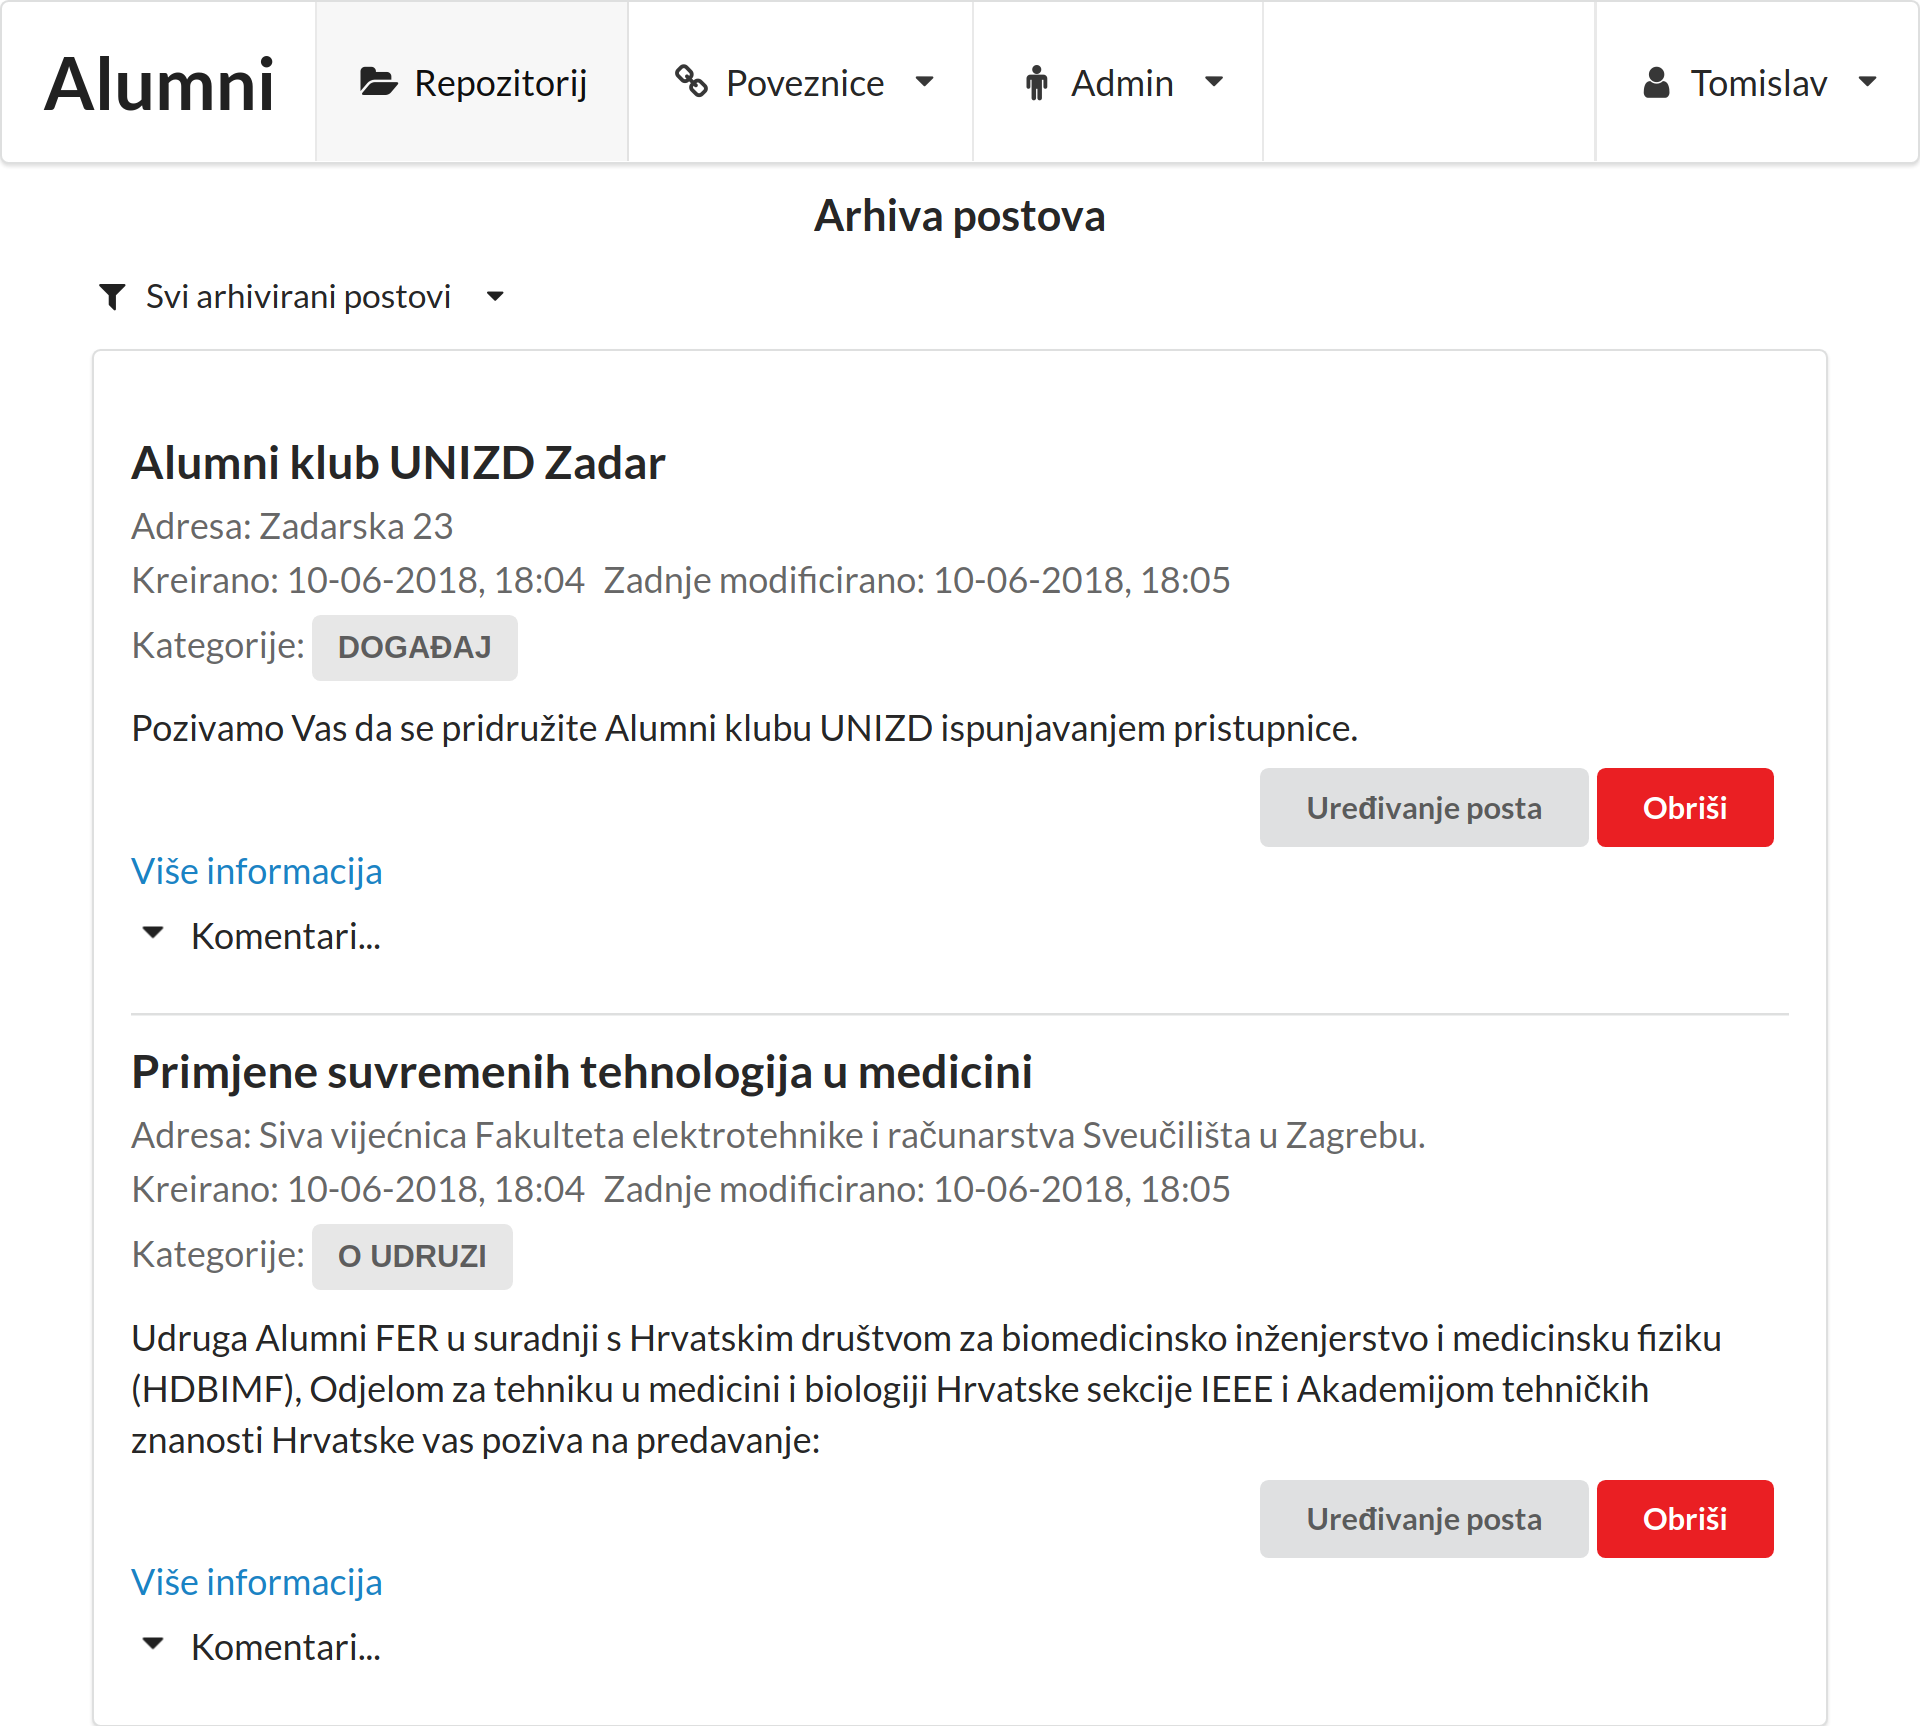
\includegraphics[width=13cm]{slike/arhivirani-postovi.png}
	\caption{Pregled arhiviranih postova}
	\label{fig:arhivirani-postovi}
\end{figure}

Do pregleda arhiviranih postova dolazi se odabirom opcije "Arhiva postova" u padajućem izborniku "Admin" na navigacijskoj traci. Arhiva postova imitira stranicu za prikaz svih postova, te je također omogućeno filtriranje, straničenje, brisanje te uređivanje tih postova.

\subsection{Komentari}

\begin{figure}[H]
	\centering
	
\includegraphics[width=13cm]{slike/komentari.png}
	\caption{Komentari na postu}
	\label{fig:komentari}
\end{figure}

Zbog toga što je ovo stranica za upravljanje zajednicom, vrlo je bitan društveni aspekt te zajednice te je vrlo bitna interakcija korisnika sa sustavom i međusobno. To je ostvareno preko sustava komentara kojim bilo koji prijavljeni korisnik može komentirati postove.

\subsubsection{Dodavanje novog komentara}

Čim je korisnik prijavljen na sustav, može komentirati na post iz pregleda svih postova, odabirom opcije "Komentari...", upisivanjem komentara u obrazac i pritiskom gumba za komentiranje. Prilikom komentiranja postoji provjera da li komentar postoji, odnosno nije moguće izraditi prazan komentar. Za svaki komentar je u pregledu komentara postova prikazan autor tog komentara, odnosno njegovo ime i prezime, datum objave tog komentara, te sadržaj komentara.

\subsubsection{Brisanje komentara}
Korisnici imaju mogućnost komentiranja bilo čega, pa ti komentari često mogu biti zlonamjerni ili neprimjereni. Zato je administratoru omogućeno brisanje komentara pomoću ikonice smeća pored datuma komentara.

\section{Sustav pretplata}
Korisnici često propuste neke važne obavijesti na stranicama ako redovno ne posjećuju te stranice. Zbog toga postoji sustav pretplata pomoću kojeg se korisnik pretplati na željene kategorije postova. Od tog trenutka nadalje, korisnik prilikom svake objave posta koji sadrži kategoriju na koju je korisnik pretplaćen, dobiva obavijest na email.

\subsection{Dodavanje i ažuriranje pretplata}

\begin{figure}[H]
	\centering
	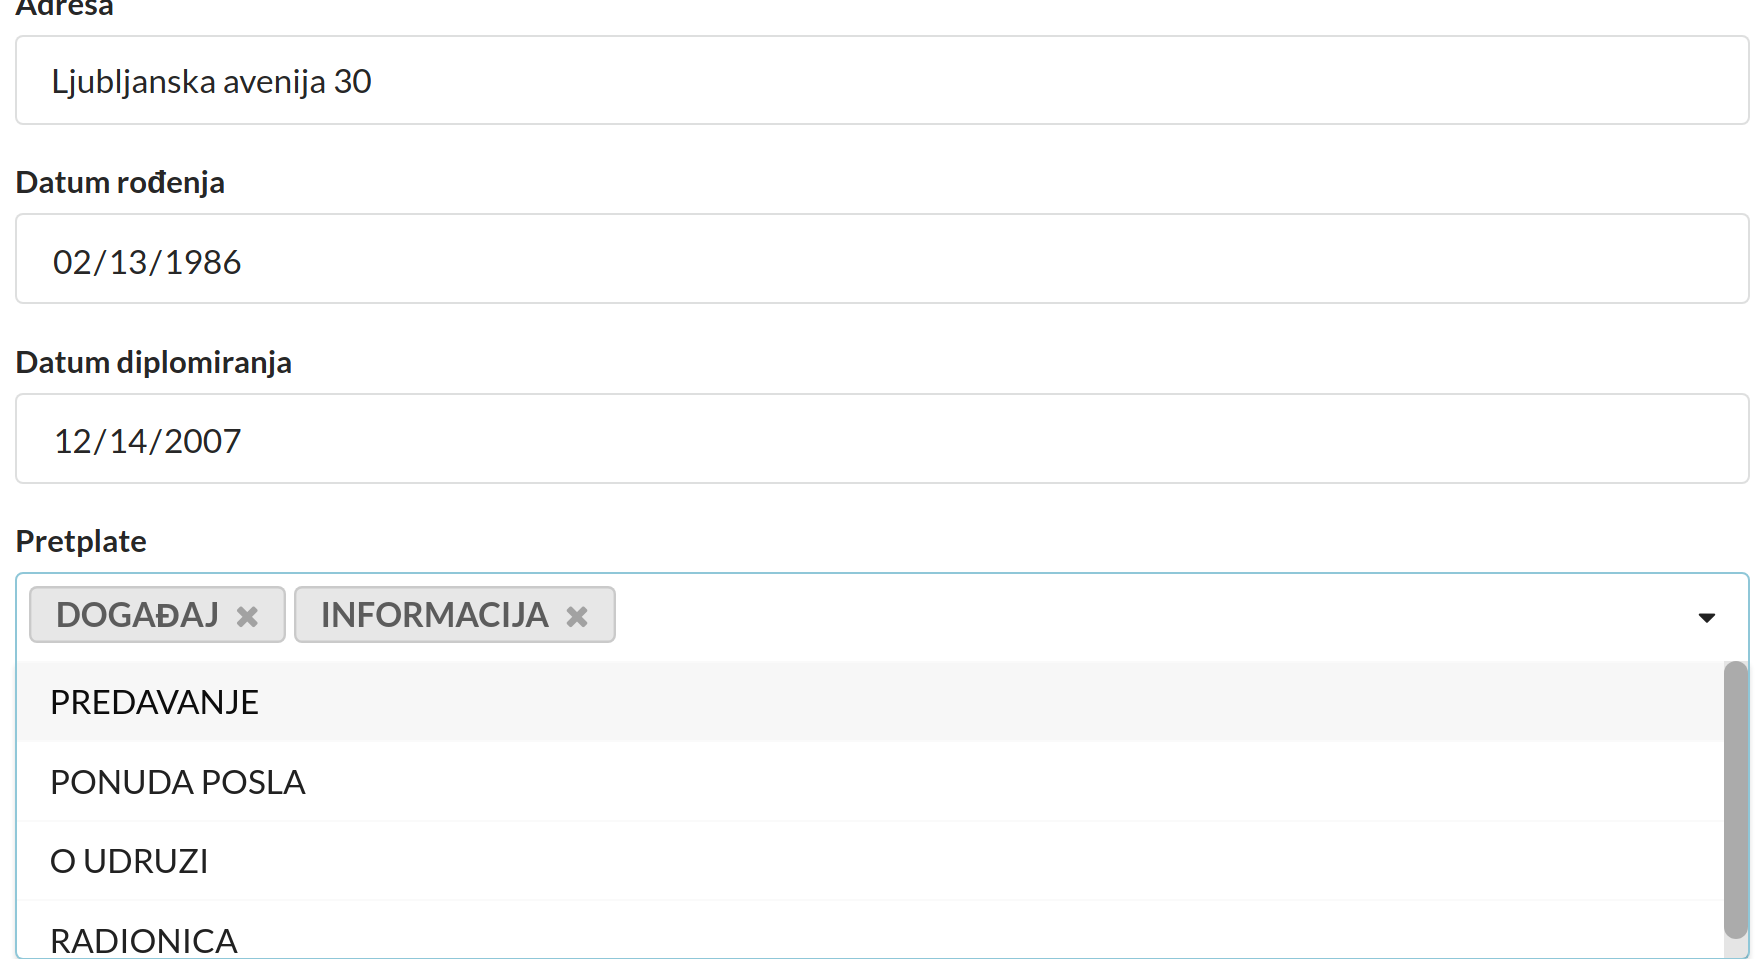
\includegraphics[width=13cm]{slike/pretplate.png}
	\caption{Dodavanje pretplata na obrascu za uređivanje korisnika}
	\label{fig:pretplate}
\end{figure}

Uređivanje pretplata ostvareno je u sklopu uređivanja korisničkog računa, pri dnu obrasca. Korisnik se pomoću više-odabirnog padajućeg izbornika može pretplatiti na određene kategorije postova. Na taj isti način mogu se i ukloniti pretplate. Korisnik ne mora nužno biti pretplaćen na bilo koju kategoriju. Ako je korisnik pretplaćen na neke kategorije, to je vidljivo na pregledu njegovog računa.

\subsection{Slanje pošte prilikom dodavanja novog posta}

\begin{figure}[H]
	\centering
	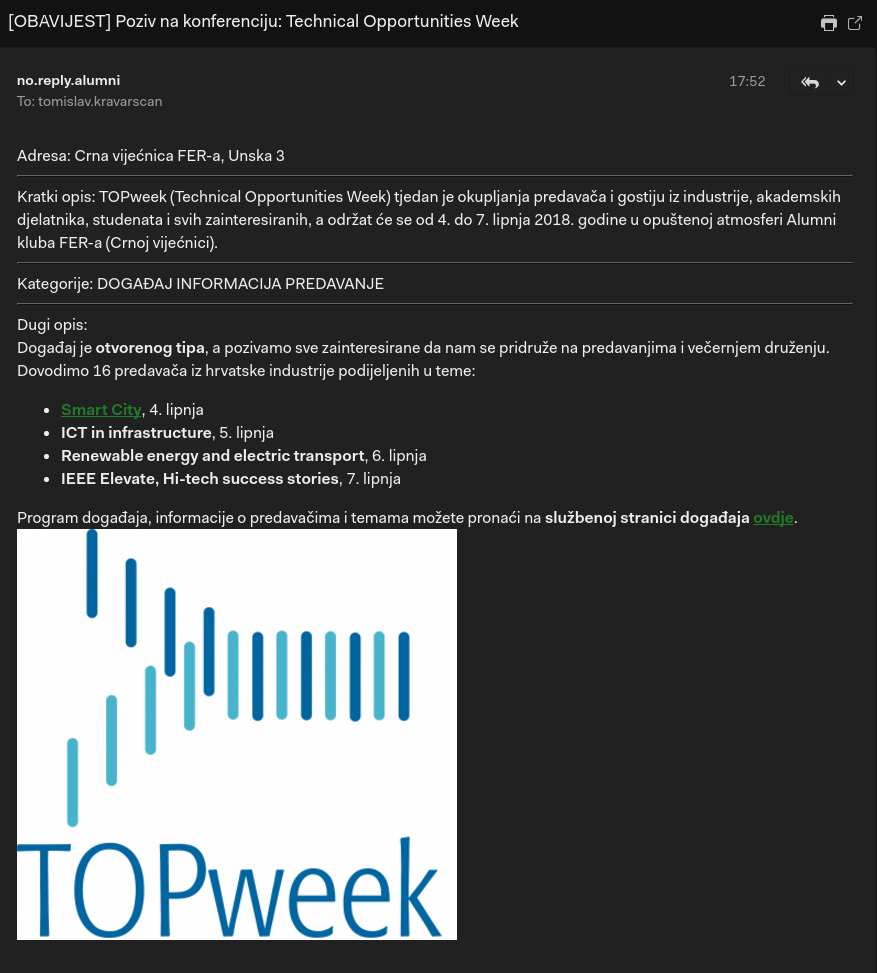
\includegraphics[width=13cm]{slike/mail.png}
	\caption{Izgled email-a obavijesti} 
	\label{fig:mail}
\end{figure}

Kada administrator na stranici izradi novi post, automatski se svim korisnicima koji su pretplaćeni na kategorije koje sadrži taj post šalje email sa cjelokupnim sadržajem tog posta. Tip sadržaja tog email-a je \textit{html} kao što je vidljivo na slici \ref{fig:mail}. 

\chapter{Korištene tehnologije i alati}

\section{Razvojni okviri}

\subsection{Maven}

\textit{Apache Maven}\citep{apache-maven} je alat za upravljanje projektom. Pomoću \textit{xml} (eng. \textit{EXtenisble Markup Language}) datoteke pom.xml (eng. \textit{Project Object Model}) upravlja projektom pomoću niza \textit{xml} oznaka. U toj datoteci nalazi se popis ovisnosti, ime aplikacije i još mnogo meta-podataka bitnih za ispravan rad. Jednostavnim dodavanjem nove ovisnosti oznakom \textit{dependency} unutar oznake \textit{dependencies}, većina radnih okruženja automatski sa interneta skine potrebne datoteke i smjesti ih u naš projekt. Ovo je vrlo važna komponenta razvoja jer bi uz toliko ovisnosti o drugim komponentama snalaženje u procesu bilo gotovo nemoguće.

\subsection{Spring}

\subsubsection{Spring Boot}
\textit{Spring Boot}\citep{spring-boot} je vrlo moćan i opširan razvojni okvir kojim se nastoji olakšati razvoj složenih aplikacija u Javi. Točnije, \textit{Spring Boot} je nadogradnja na već postojeći okvir \textit{Spring},koji ima nedostatak u procesu razvoja u obliku vrlo opširne i naporne konfiguracije kako bi se dobilo radno rješenje. \textit{Spring Boot} je po svim funkcionalnostima isti kao \textit{Spring}, ali je početno postavljanje i konfiguriranje projekta svedeno na minimum. Radna verzija okvira se može dobiti automatskim generiranjem preko \textit{Spring Initializr}\citep{spring-initializr} alata, gdje se upišu željeni meta-podaci i dodaju ovisnosti o drugim projektima preko obrasca na službenoj stranici. Dodatne datoteke za konfiguraciju mogu se po volji izrađivati, a glavna je \textit{application.properties}, u kojoj se nalaze neke osnovne karakteristike kao što je port na kojem će aplikacija slušati.

\subsubsection{Spring Security}
\textit{Spring Security}\citep{spring-security} jedna je od korištenih nadogradnji na osnovni \textit{Spring} projekt. Pomoću njega moguće je jednostavno stvoriti sustav autorizacije i autentifikacije, definirati ograničenja na pristupanje upravljačima i njihovim metodama te spriječiti stvaranje određenih elemenata neautoriziranim korisnicima na pogledima. Prema \textit{Pivotal Software}-u, ovo je standardni način osiguravanja aplikacije u \textit{Spring} projektu.

\subsection{Java Persistance API}
\textit{Java Persistance API - JPA}\citep{jpa} je specifikacija sučelja koja opisuje upravljanje relacijskim podacima unutar aplikacije u Javi. To je skup konvencija kojih bi se svi koji žele implementirati ORM (eng. \textit{Object Relation Model}) trebali pridržavati.

\subsubsection{Hibernate ORM}
\textit{Hibernate ORM}\citep{hibernate} je implementacije JPA sučelja koja je vrlo intuitivna za korištenje te ima vrlo dobre performanse. Bazirana je na \textit{code-first} načinu programiranja, gdje se programer ne brine oko implementiranja baze podataka, nego izrađuje modele podataka izravno u Java razredima i u isto vrijeme se posebnim oznakama, odnosno anotacijama definira izgled tablica u bazi. To također i olakšava dohvaćanje entiteta iz baze pomoću razreda koji oponašaju repozitorije, odnosno preko metoda u Javi pružaju apstraktan pogled na \textit{query} naredbe u bazi. Kod izrade razreda repozitorija programer nasljeđuje \textit{JPARepository} razred, u kojem su već predefinirane neke metode koje se najčešće koriste prilikom dohvata podataka, kao npr. \textit{jpa.findAll()} metoda koja dohvaća sve podatke iz neke tablice.

\subsection{JavaServer Pages}
\textit{Java Server Pages - JSP}\citep{jsp} nam omogućava stvaranje pogled, odnosno web stranica koje imaju statične - običan html i dinamične elemente. Dinamični elementi se definiraju JSP oznakama, a mogućnosti su vrlo opširne. Dinamičnost elemenata postiže se izvršavanjem koda ubačenog u JSP stranicu na poslužiteljskom dijelu aplikacije. Taj kod, osim oznake, može biti i običan Java kod.

\subsection{JavaScript}
\textit{JavaScript} je implementacija \textit{ECMAScipt}\citep{ecma-script} specifikacije. To je skriptni, interpretirani jezik koji koriste web preglednici. On nam omogućuje izradu vrlo dinamičnih stranica i vrlo je fleksibilan. Program napisan u JavaScriptu se izvodi na klijentskoj strani aplikacije. Pomoću njega možemo manipulirati DOM-om (eng. \textit{Document Object Model}) html stranice. Uz HTML i CSS (eng. \textit{Cascading Style Sheets}), JavaScript je jedna od tri glavnih tehnologija korištenih na internetu u web preglednicima. Bitna tehnika u programskom jeziku JavaScript je AJAX (eng. \textit{Asynchronous JavaScript And XML}), kojim možemo komunicirati sa web poslužiteljem i nakon što je stranica učitana. To čini izmjenjivanjem XML dokumenata sa poslužiteljem, iako se u današnjici gotovo stalno koristi JSON notacija (eng. \textit{JavaScript Object Notation}). 

\subsubsection{JQuery}
\textit{JQuery}\citep{jquery} je mala i brza JavaScript biblioteka. On olakšava upotrebu JavaScripta smanjivanjem potrebnih linija koda. Također ga podržava većina modernih web preglednika te je intuitivan za korištenje.

\subsection{SemanticUI}
Html stranice same po sebi nisu baš oku ugodne, samo su funkcionalne. Kako bi se stranica uljepšala koristi se CSS, kojim možemo definirati razne karakteristike elemenata na stranici kao što su boja, veličina, granice. CSS je vrlo opširan i na izgledu stranice može se potrošiti dosta vremena. Ako želimo da nam stranica pristojno izgleda, ali nemamo baš vremena, možemo koristiti neke CSS biblioteke koje imaju dobar odziv na različite vrste uređaja (npr. prilagode se ekranu mobitela). Jedna od takvih bibilioteka je \textit{SemanticUI}\citep{semantic}, koji programer koristi korištenjem postojećih imena razreda za svaku html oznaku na stranici. SemanticUI je besplatan i otvorenog koda, pod MIT licencom.

\section{Baza podataka}
Baza korištena u ovoj aplikaciji je također besplatna i otvorenog koda, \textit{MySQL}\citep{mysql}. To je relativno nova i brza relacijska baza podataka koja je dobar izbor jer je optimizirana za web aplikacije, štoviše, na neki način je postala standardnom bazom za internetski orijentirane aplikacije. Sa ovom aplikacijom se spaja preko JDBC-a (eng. \textit{Java Database Connectivity}), koja definira način na koji klijent pristupa bazi.

\section{Razvojno okruženje}
\textit{Visual Studio Code - VSCode}\citep{vscode} je lakša verzija okruženja \textit{Visual Studio}, koja ne pruža mnogo funkcionalnsti sama po sebi, ali je napravljena tako da je moguće dodati proširenja po želji. Proširenja pišu korisnici i nije ih komplicirano napraviti. Osim toga, VSCode je podržan na mnogim operacijskim sustavima, za razliku od Visual Studia.



\chapter{Zaključak}
Ovom se aplikacijom uz vrlo jednostavno sučelje može informirati svršenike neke organizacije o bitnim događajima ili bilo kakvim drugim vrstama objava zbog sustava postova i pretplata. Također, upravljanje korisničkim računima osigurava administratorima koji upravljaju zajednicom uvid u aktivnost korisnika aplikacije. Aplikacija kao vrlo važan aspekt sustava uzima sigurnost korisničkih podataka te samo ovlaštene osobe imaju pristup određenim dijelovima sustava, što je vrlo bitno za krajnjeg korisnika.

Korisnici mogu biti u interakciji sa administratorima, sustavom drugim korisnicima preko komentara na postove, što je, osim pregleda vijesti, vrlo korisno.

\bibliography{literatura}
\bibliographystyle{fer}

\begin{sazetak}
	Rad obuhvaća teorijski dio potreban za razumijevanje potrebe za aplikacijom kojom bi se upravljalo svršenicima, zatim implementaciju takve aplikacije i popratnu dokumentaciju u obliku funkcionalnosti i arhitekture sustava kojom je ostvareno.
	
	Za uspješan rad takve aplikacije, osnovne mogućnosti koje je potrebno imati su objave vijesti, pregled korisnika, definiranje specifičnih kategorija za vlastitu zajednicu svršenika te sustav pretplata kojim korisnik obavijesti dobiva email-om.
	
	\kljucnerijeci{Aplikacija, programska podrška, vijesti, korisnici, kategorije, pretplate, obavijesti, internet, klijent, poslužitelj}
\end{sazetak}

% TODO: Navedite naslov na engleskom jeziku.
\engtitle{Alumni menagement software}
\begin{abstract}
	This paper explains the theory behind the necessity of an application for menaging alumnae, then, it explains the implementation of such software and that software's documentation in form of functionalities it has and the architecture of its system.

	For this application to be successful, there are some core features that ought to be implemented such as posting news, overview of its users, defining a specific category relevant for an alumnae community and subscription system that allows user to read notification for a posted news via email.
			
	\keywords{Application, software, news, users, categories, subscriptions, notifications, web, client, server}
\end{abstract}

\end{document}
